\chapter{Supplementary Material for Contribution 2 (RQ2)}\label{app:rq2}

\section{Extended Nomenclature}\label{app:rq2_nomenclature}

Table~\ref{tab:nomenclature_rq2} lists the extended nomenclature for the transport sector decarbonization model described in Section~\ref{sec:rq2_results}.

\begin{scriptsize}
\begin{longtable}{llll}
\caption{Extended nomenclature for the transport sector decarbonization model (RQ2).}
\label{tab:nomenclature_rq2}\\
\hline
Sets and indices & Description & & \\ \hline
\endfirsthead
\endhead
\hline
\endfoot
\endlastfoot
$y \in \mathcal{Y}$ & year & & \\
$u \in \mathcal{U}$ & consumer group & & \\
$p \in \mathcal{P}$ & trip purpose & & \\
$r \in \mathcal{R}_p$ & \begin{tabular}[t]{@{}l@{}}trip between origin-destination (OD) pair\\ for a specified purpose\end{tabular} & & \\
$k \in \mathcal{K}$ & travel paths & & \\
$e \in \mathcal{E}$ & geographic location & & \\
$v \in \mathcal{V}$ & type of vehicle & & \\
$t \in \mathcal{T}_v$ & \begin{tabular}[t]{@{}l@{}}drive-train technology fueled\\ by a specific fuel\end{tabular} & & \\
$g \in \mathcal{G}$ & year that vehicle was introduced to market & & \\
$l \in \mathcal{L}$ & \begin{tabular}[t]{@{}l@{}}types of fueling infrastructure\\ (by capacity)\end{tabular} & & \\
$i \in \mathcal{I}_l$ & \begin{tabular}[t]{@{}l@{}}index for detour time reduction potential\\ for type of fueling infrastructure $l$\end{tabular} & & \\
$\mathcal{Y}^{exp}$ & set of years of investment decisions & & \\
$\mathcal{K}_{e}$ & set of paths that go through edge $e$ & & \\
$\mathcal{L}^{not home}$ & \begin{tabular}[t]{@{}l@{}}fueling infrastructure that is not allocated\\ at home of vehicle owner\end{tabular} & & \\
$\mathcal{L}^{home}$ & \begin{tabular}[t]{@{}l@{}}fueling infrastructure that is allocated\\ at home of vehicle owner\end{tabular} & & \\
$\mathcal{L}_{tk}$ & \begin{tabular}[t]{@{}l@{}}types of infrastructure by drive-train\\ technology and availability for travel path\end{tabular} & & \\
$\mathcal{E}_{kl}$ & \begin{tabular}[t]{@{}l@{}}geographic location along travel path\\ and available fueling type\end{tabular} & & \\
$S^u_j$ & \begin{tabular}[t]{@{}l@{}}subsets of time periods for which a monetary\\ budget is defined by consumer group\end{tabular} & & \\
\\\hline
Decision variables & Description & Unit & Domain \\ \hline
$f_{yurkvtg}$ & number of person-trips & -- & $[0,\infty[$ \\
$h_{yurkvtg}$ & number of vehicles & -- & $[0, \infty[$ \\
$h^{+}_{yurkvtg}$ & newly purchased vehicles & -- & $[0,\infty[$ \\
$h^{-}_{yurkvtg}$ & \begin{tabular}[t]{@{}l@{}}number of vehicles leaving\\ the vehicle stock\end{tabular} & -- & $[0, \infty[$ \\
$s_{yurkvtgle}$ & energy fueled & kWh & $[0, \infty[$ \\
$n_{yurkvtgle}$ & number of fueling vehicles & -- & $[0, \infty[$ \\
$b_{yurkvtle}$ & \begin{tabular}[t]{@{}l@{}}fueling detour time to reach closest\\ available public charging infrastructure\end{tabular} & h & $[0, \infty[$ \\
$w_{yeli}$ & \begin{tabular}[t]{@{}l@{}}binary decision variable indicating whether\\ detour reduction $i$ is active\end{tabular} & -- & $\{0, 1\}$ \\
$z_{yrkvtle,i}$ & \begin{tabular}[t]{@{}l@{}}decision variable substituting\\ the multiplication $b \times w$\end{tabular} & h & $[0, \infty[$ \\
$q^{+,\mathrm{fuel\_infr, home}}_{yrte}$ & added fueling infrastructure at home & kW & $[0,\infty[$ \\
$q^{+, \mathrm{fuel\_infr}}_ {ytle}$ & added fueling infrastructure & kW & $[0, \infty[$ \\
$q^{\Delta +, \mathrm{fuel\_infr}}_ {ytle}$ & \begin{tabular}[t]{@{}l@{}}relative difference of fueling capacity\\ expansion to fixed capacity size values\end{tabular} & kW & $[0, \infty[$ \\
$\mathrm{budget}^{+}_{yur}$ & budget overrun & \euro & $[0, \infty[$ \\
$\mathrm{budget}^{-}_{yur}$ & budget underrun & \euro & $[0, \infty[$ \\
\\\hline
Parameters & Description & Unit & Domain \\ \hline
$\mathrm{LoS}$ & level of service & h & $[0, \infty[$ \\
$\mathrm{VoT}$ & value of time & \euro/h & $[0, \infty[$ \\
$\gamma_l$ & \begin{tabular}[t]{@{}l@{}}factor between annual peak hour\\ and total annual demand\end{tabular} & \% & $[0, 100]$ \\
$Q^{\mathrm{fuel\_infr, not home}}_{urte}$ & initial fueling infrastructure (not home) & kW & $[0, \infty[$ \\
$Q^{\mathrm{fuel\_infr, home}}_{urtle}$ & initial fueling infrastructure at home & kW & $[0, \infty[$ \\
$\hat{Q}^{\mathrm{max}}_{yule}$ & \begin{tabular}[t]{@{}l@{}}upper limit for charging infrastructure\\ capacity by consumer group\end{tabular} & kW & $[0, \infty[$ \\
$\hat{Q}^{\mathrm{max}}_{yle}$ & \begin{tabular}[t]{@{}l@{}}upper limit for charging\\ infrastructure capacity\end{tabular} & kW & $[0, \infty[$ \\
$\alpha_{iel}$ & reduction $i$ of detour time & \% & $[0, 100]$ \\
$cap_{eli}$ & \begin{tabular}[t]{@{}l@{}}fixed lower bounds for capacity which tie\\ to a reduction of detour time of $\alpha_{i}$\end{tabular} & kWh & $[0, \infty[$ \\
$\tau^u$ & \begin{tabular}[t]{@{}l@{}}vehicle replacement period\\ by consumer group\end{tabular} & a & $[0, \infty[$ \\
$\beta$ & \begin{tabular}[t]{@{}l@{}}relative threshold for budget\\ under- or overrun\end{tabular} & \% & $[0, 100]$ \\
$B^{\mathrm{init}}_{el}$ & initial detour time & h & $[0, \infty[$ \\
$D^{\textrm{spec}}_{vtg}$ & specific energy consumption & kWh/km & $[0, \infty[$ \\
$W_{vtg}$ & load factor & persons/vehicle & $[0, \infty[$ \\
$\mathrm{Cap}^{\mathrm{tank}}_{vtg}$ & tank capacity & kWh & $[0, \infty[$ \\
$L^{annual}_{vtg}$ & annual range & km & $[0, \infty[$ \\
$L_{k}$ & length of path & km & $[0, \infty[$ \\
$C^{\mathrm{CAPEX}}_{yvtg}$ & expenditure costs for vehicles & \euro & $[0, \infty[$ \\
$\mathrm{Budget}_u$ & monetary budget of consumer group & \euro/trip & $[0, \infty[$ \\
\hline
\end{longtable}
\end{scriptsize}

\section{Extended Mathematical Formulation}\label{app:rq2_math}

This section provides the extended set of constraints of the transport sector decarbonization model.

\textbf{Demand coverage:}
\begin{equation} \label{equ:demand_cov}
    \begin{split}
        \sum_{k \in \mathcal{K}_r} \sum_{v \in V} \sum_{t \in \mathcal{T}_v} \sum_{g \in \mathcal{G}} f_{yurkvtg} = F_{yur} \quad :  \forall y, u, r
    \end{split}
\end{equation}

\textbf{Fleet sizing:}
\begin{flalign} \label{equ:fleet_size_demand}
    \begin{split}
         h_{yurvtg} \geq \sum_{k \in \mathcal{K}_r}\frac{L_{k}}{W_{yvtg} L^{\mathrm{annual}}_{vtg}} f_{yurkvtg} \quad :\forall y,u,r,k,v,t,g
    \end{split}
\end{flalign}

\begin{flalign} \label{equ:fleet_size_change_1}
    \begin{split}
         \sum_{p} h_{yurvtg} = \sum_{p} h_{(y-1)rvtg} + \sum_{p} h^{+}_{yurvtg} - \sum_{p} h^{-}_{yurvtg} \quad :\forall y\in \mathcal{Y}\setminus{\{0\}},u,r,v,t,g
    \end{split}
\end{flalign}

\begin{flalign} \label{equ:fleet_size_change_2}
    \begin{split}
         \sum_{p}  h^{-}_{yurvt(g=y-\textrm{Lifetime}^{max}_{vtg})} =\sum_{p}  h_{yrvt(g=y-\textrm{Lifetime}_{vtg})} \quad: \forall y,u,r,v,t
    \end{split}
\end{flalign}

\textbf{Fueling demand:}
\begin{flalign} \label{equ:fuel_demand}
    \begin{split}
        \sum_{l \in \mathcal{L}_{tk}} \sum_{e \in \mathcal{E}_{kl}} s_{yurkvtgle} \geq \sum_{e \in \mathcal{E}_{k} }  \gamma_l \frac{D^{\mathrm{spec}}_{gvt}}{W_{gvt}L_{k}} f_{yurkvtg}: \forall y,u,r,k,v,t,g
    \end{split}
\end{flalign}

\textbf{Number of fueling vehicles:}
\begin{flalign}
    \begin{split}
        \sum_{v,t} \frac{1}{\textrm{Cap}^{\mathrm{tank}}_{vtg}}s_{yurkvtgle} = n_{yurklge} \quad : \forall y,u,r,k,g,e, l \in \mathcal{L}^{vt}
    \end{split}
\end{flalign}

\textbf{Maximum capacity constraints:}
\begin{flalign}
    \begin{split}
        Q^{\mathrm{fuel\_infr}}_{tle} + \sum_{y' \in \mathcal{Y}^{\mathrm{exp}}_y} q^{+, \mathrm{fuel\_infr}}_{ytle} \leq \hat{Q}^{\mathrm{fuel\_infr}}_{tle} \quad : \forall y, t, l, e \\
        \sum_{r \in \mathcal{R}_u} \left( Q^{\mathrm{fuel\_infr, home}}_{urtle}  + \sum_{y' \in \mathcal{Y}^{\textrm{exp}}_y} q^{+, \mathrm{fuel\_infr, home}}_{yurtle} \right)\leq \hat{Q}^{\mathrm{fuel\_infr,home}}_{utle} : \forall y, u, t, l, e
    \end{split}
\end{flalign}

\section{Pre-processing of Travel Data}\label{app:rq2_travel_data}

The trip data used in the case study is based on Austrian mobility survey data. Trip lengths were segregated by urban and rural context, using Vienna values for urban areas and suburban values for rural areas \citep{tomschy2016osterreich}.

The clustering of trips to vehicles introduces a constraint linking commuting and private vehicle stocks. This constraint ensures consistency between the number of vehicles used for commuting and private purposes within the same geographic region:
\begin{flalign}
    \begin{split}
         \zeta_1 h_{yur(p=\textrm{commuting})kvtg} \leq  \zeta_2 h_{yur(p=\textrm{private})kvtg} \quad :\forall y, u, k, v, t, g,  r \in \mathcal{R}^{m},  m = 1, 2, \dots, M
    \end{split}
\end{flalign}

Table~\ref{tab:ratio_zeta_rq2} displays the parameter values by region.

\begin{table}[H]
\centering
\caption{Parameter setting for the relationship between number of vehicles used for commuting and private purposes by region.}
\label{tab:ratio_zeta_rq2}
\begin{tabular}{@{}lrrr@{}}
\toprule
Parameter & \multicolumn{1}{l}{Bizkaia} & \multicolumn{1}{l}{Araba} & \multicolumn{1}{l}{Gipuzkoa} \\ \midrule
$\zeta_1$ & 1 & 1 & 1 \\
$\zeta_2$ & 0.86 & 0.85 & 1.05 \\ \bottomrule
\end{tabular}
\end{table}

\section{Discretization of the Detour-Fueling Function}\label{app:rq2_discretization}

To introduce the relationship between installed charging infrastructure capacity and the detouring time to the closest available charging station into the mixed-integer linear program, the continuous detour-fueling function is discretized into piecewise steps. This discretization balances the trade-off between the loss of information due to discretization and the increase in model complexity (number of binary variables) with finer resolution. Figure~\ref{fig:dtf_sampling_rq2} illustrates the sampling of the detour fueling time functions used in the MILP formulation.

\begin{figure}[H]
    \centering
    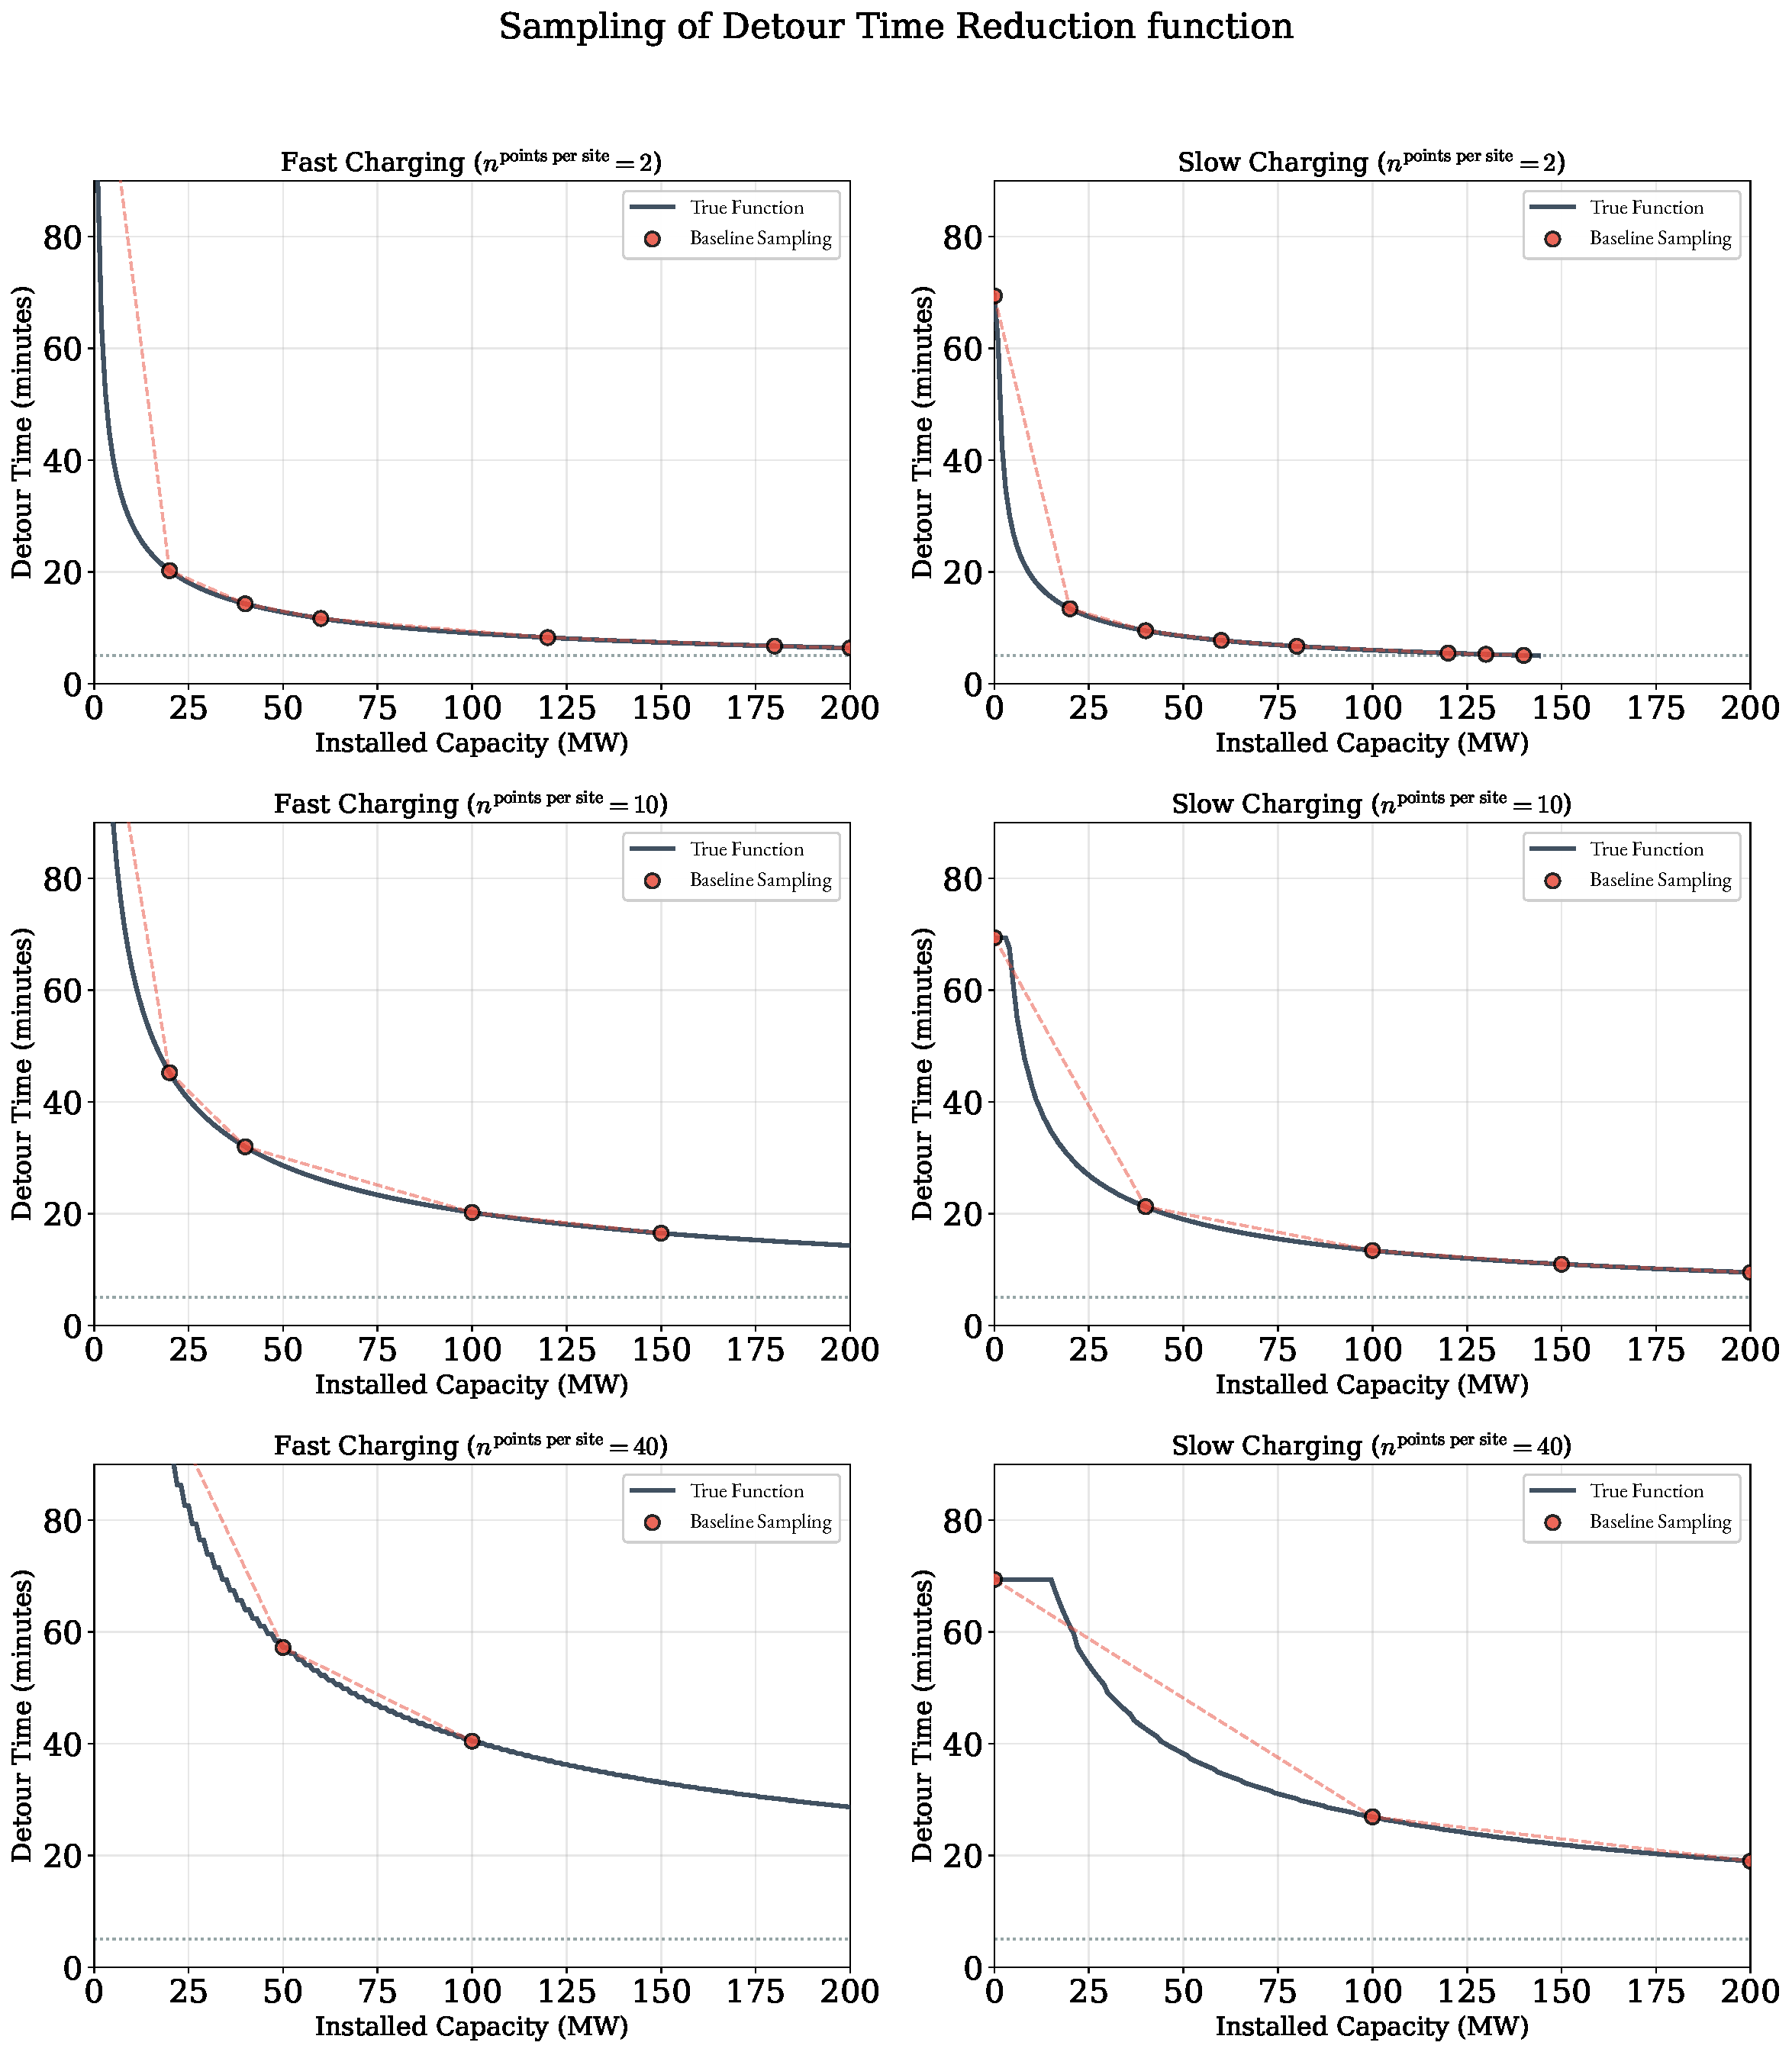
\includegraphics[width=\textwidth]{graphics/paper_2/dtf_sampling.pdf}
    \caption{Sampling of the detour fueling time functions to introduce the relation between charging infrastructure capacity expansion and detour fueling time to the MILP.}\label{fig:dtf_sampling_rq2}
\end{figure}

\section{Computational Details}\label{app:rq2_computational}

The model is implemented in Julia using JuMP~1.9 \citep{Lubin2023} and solved with Gurobi~12.0 \citep{gurobi}. Simulations are performed on an AMD Ryzen Threadripper 7980X (64 cores, 3.20~GHz base clock, 5.2~GHz boost) with 512~GB RAM.

The source code and input data are publicly available at: \url{https://github.com/antoniamgolab/iDesignRES_transcompmodel}.

\section{Sensitivity Analysis: Circuity Factor}\label{app:rq2_circuity}

A sensitivity analysis is conducted on the circuity parameter $\mu$, which translates the aerial distance to the driving distance in the road network. The tested range is $\mu \in \{1.0, 1.2, 1.4, 1.6, 1.8, 2.0, 2.2, 2.4\}$. The base case uses $\mu = 1.4$, which aligns with circuity values reported for European cities \citep{COSTA2025106087} and non-urban road networks \citep{f10121147}. Figure~\ref{fig:circuity_ass_rq2} displays the circuity values used as reference.

\begin{figure}[H]
    \centering
    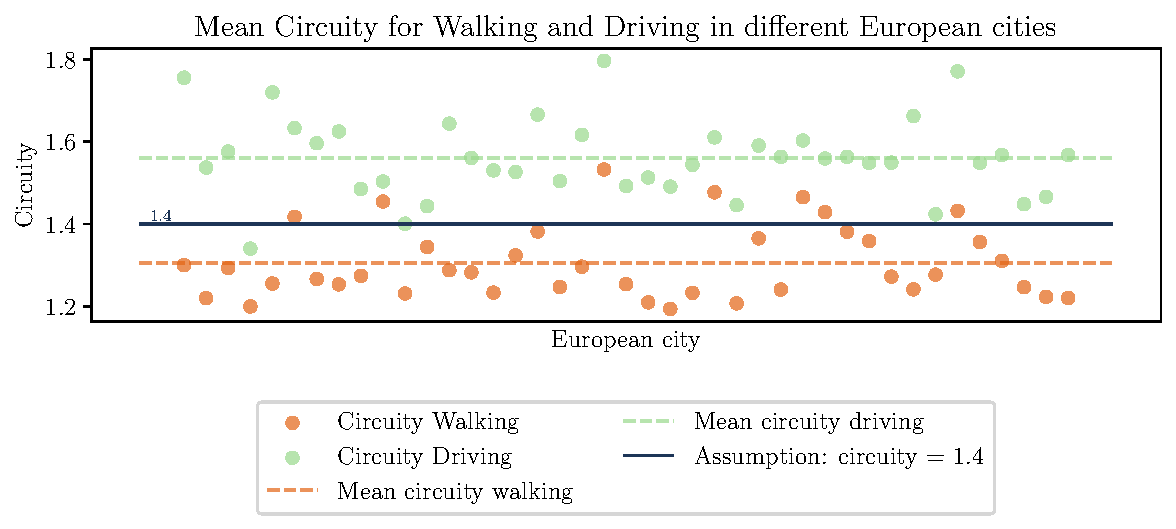
\includegraphics[width=0.8\textwidth]{graphics/paper_2/mean_circuity_plot.pdf}
    \caption{Circuity values for European cities published by \citet{COSTA2025106087}.}\label{fig:circuity_ass_rq2}
\end{figure}

Figure~\ref{fig:SA_bev_adoption_rq2} displays the distribution of electrification shares across the tested circuity values. No direct correlation is found between the increase of $\mu$ and either utilization or adoption by income class level.

\begin{figure}[H]
    \centering
    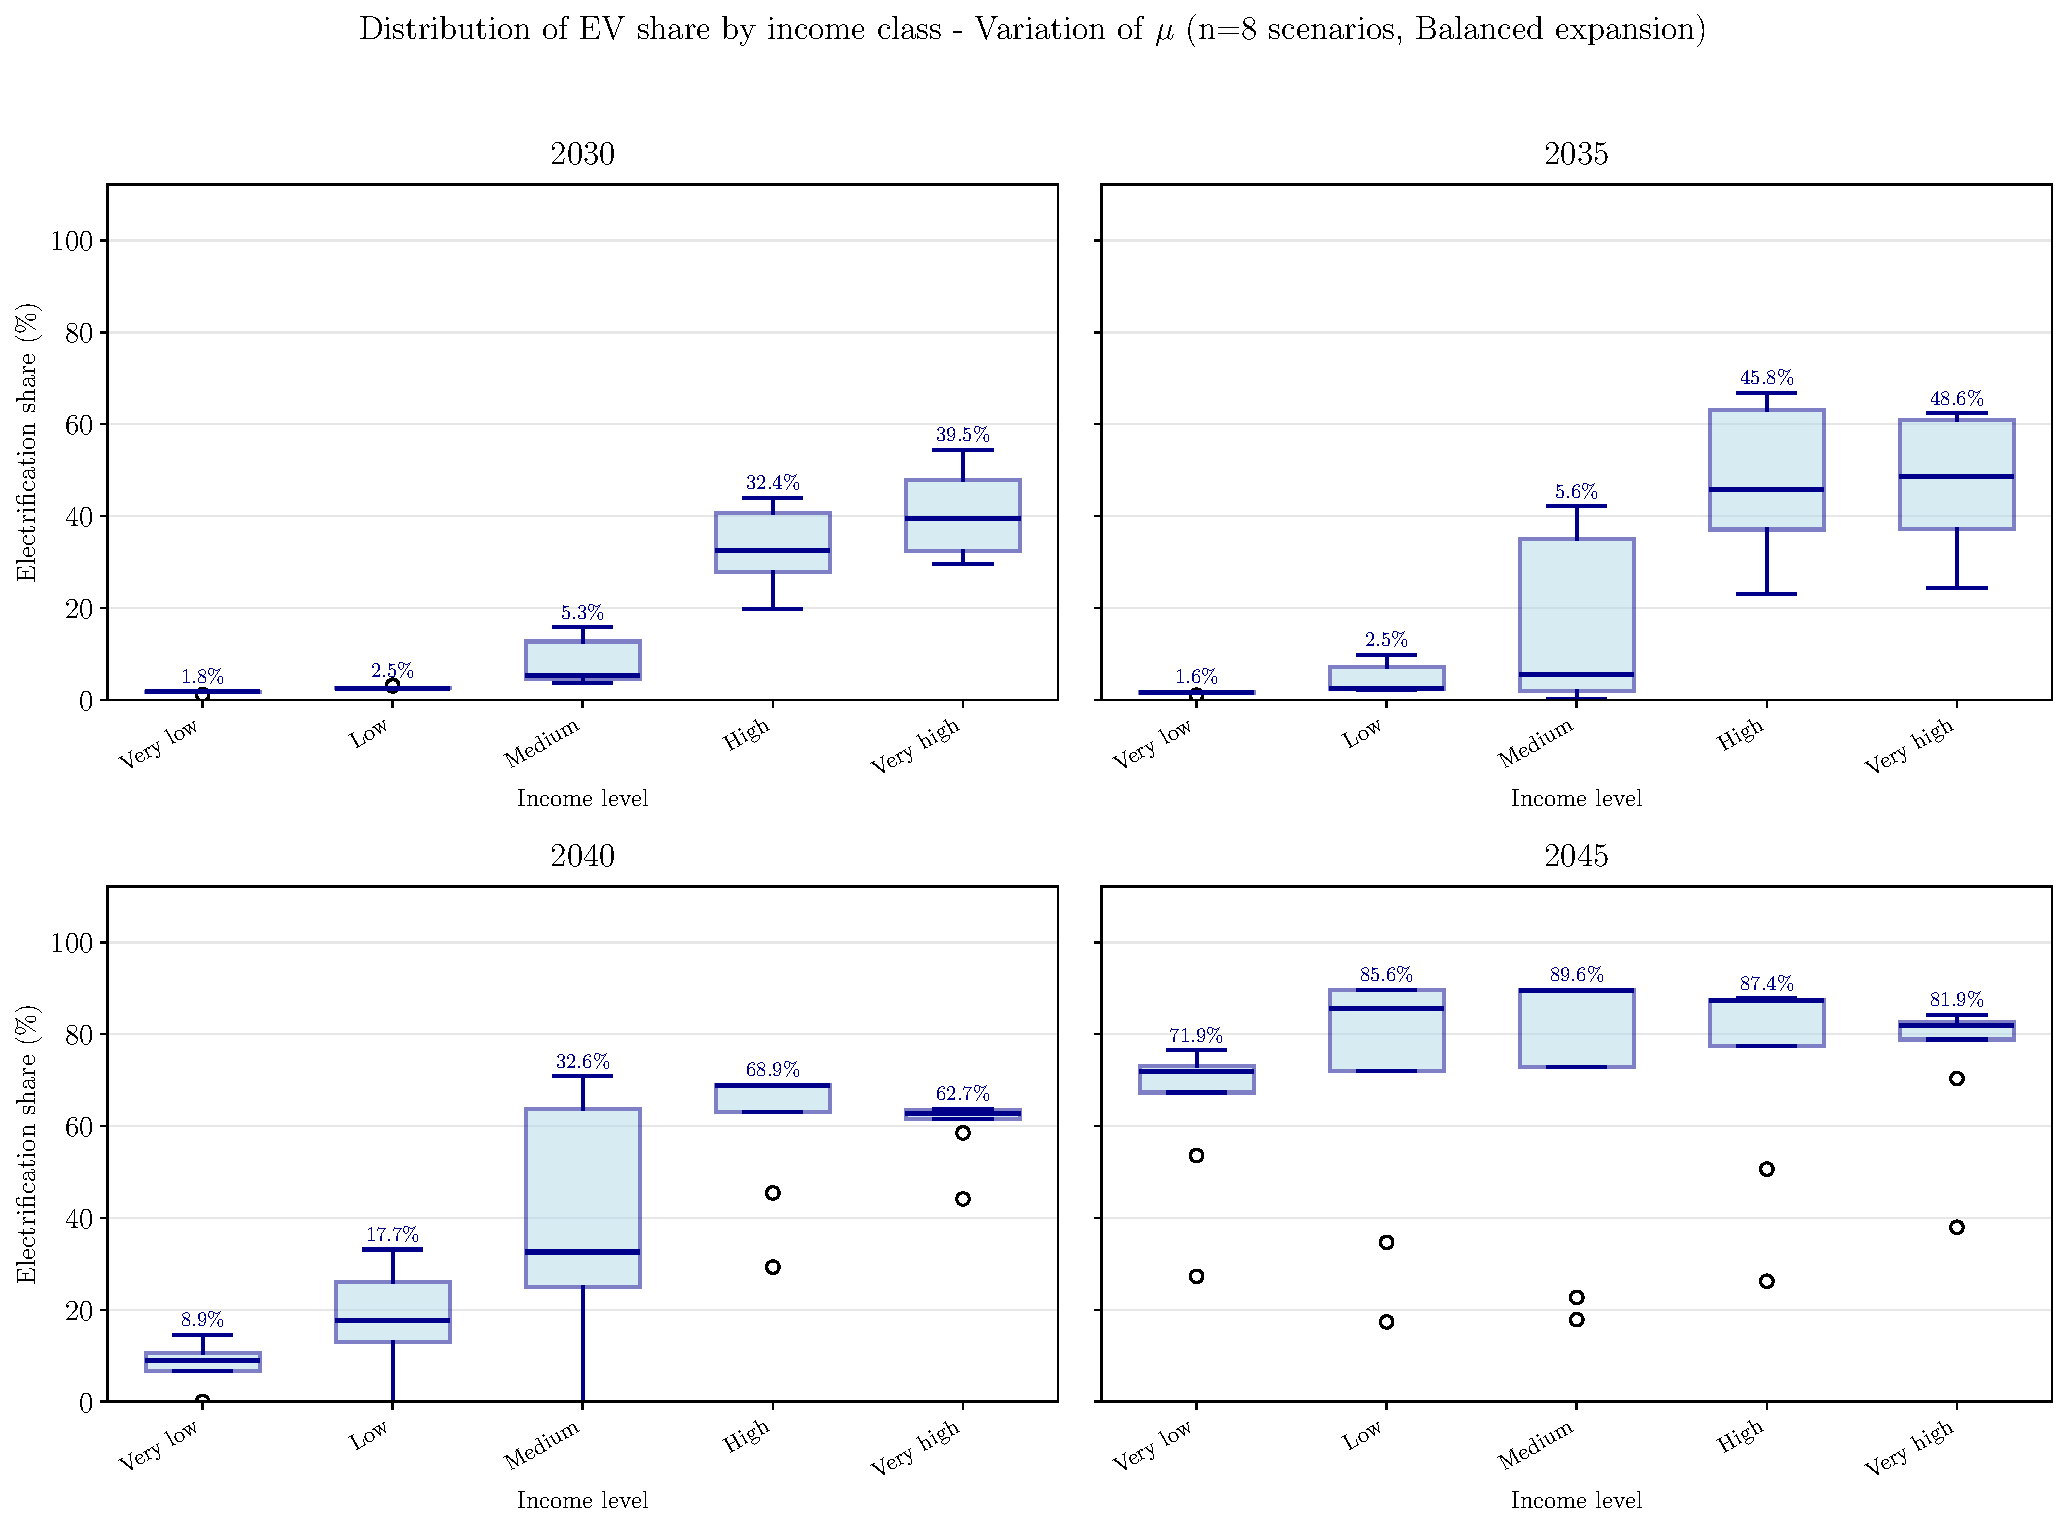
\includegraphics[width=\textwidth]{graphics/paper_2/SA_alpha_boxplot_electric_vehicles_balanced_2026.pdf}
    \caption{Distribution of the development of electrification of the passenger car fleet by income levels for different circuity values $\mu$.}\label{fig:SA_bev_adoption_rq2}
\end{figure}

\begin{figure}[H]
    \centering
    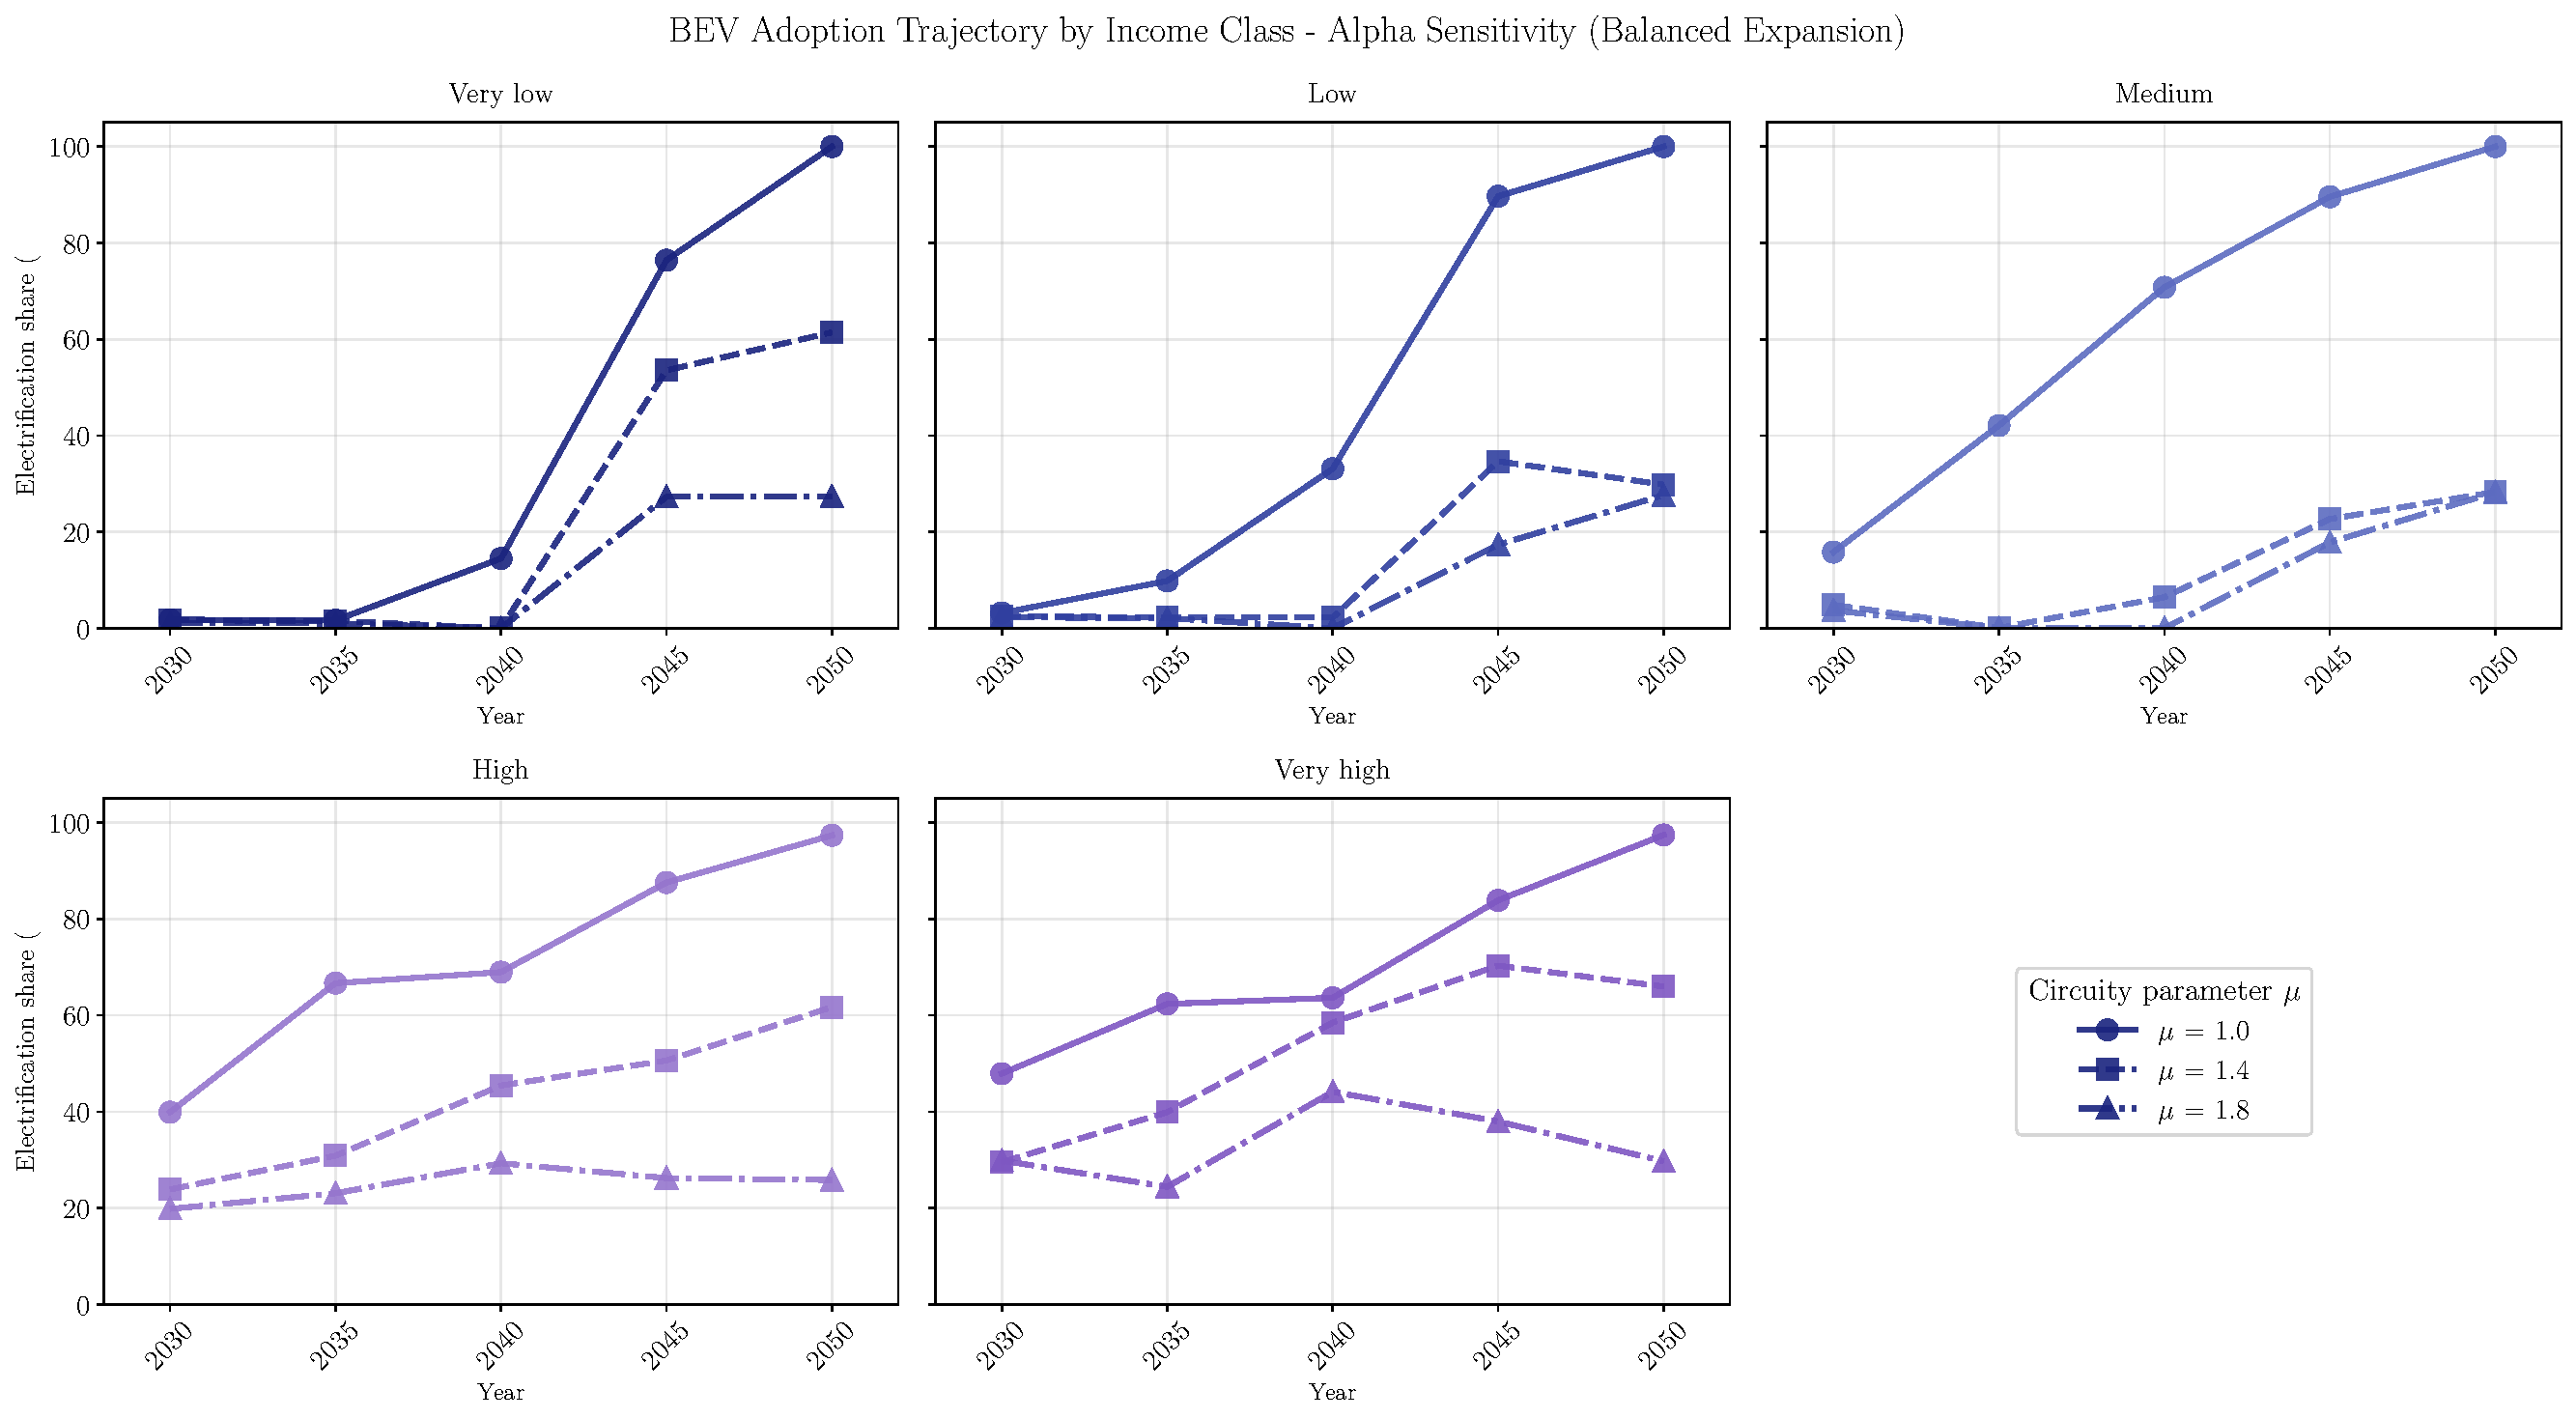
\includegraphics[width=\textwidth]{graphics/paper_2/SA_alpha_bev_shares_trajectory_by_income_2026.pdf}
    \caption{Development of electrification shares of the passenger car fleet by income classes for different parameters of $\mu$.}\label{fig:SA_alpha_dev_rq2}
\end{figure}

\begin{figure}[H]
    \centering
    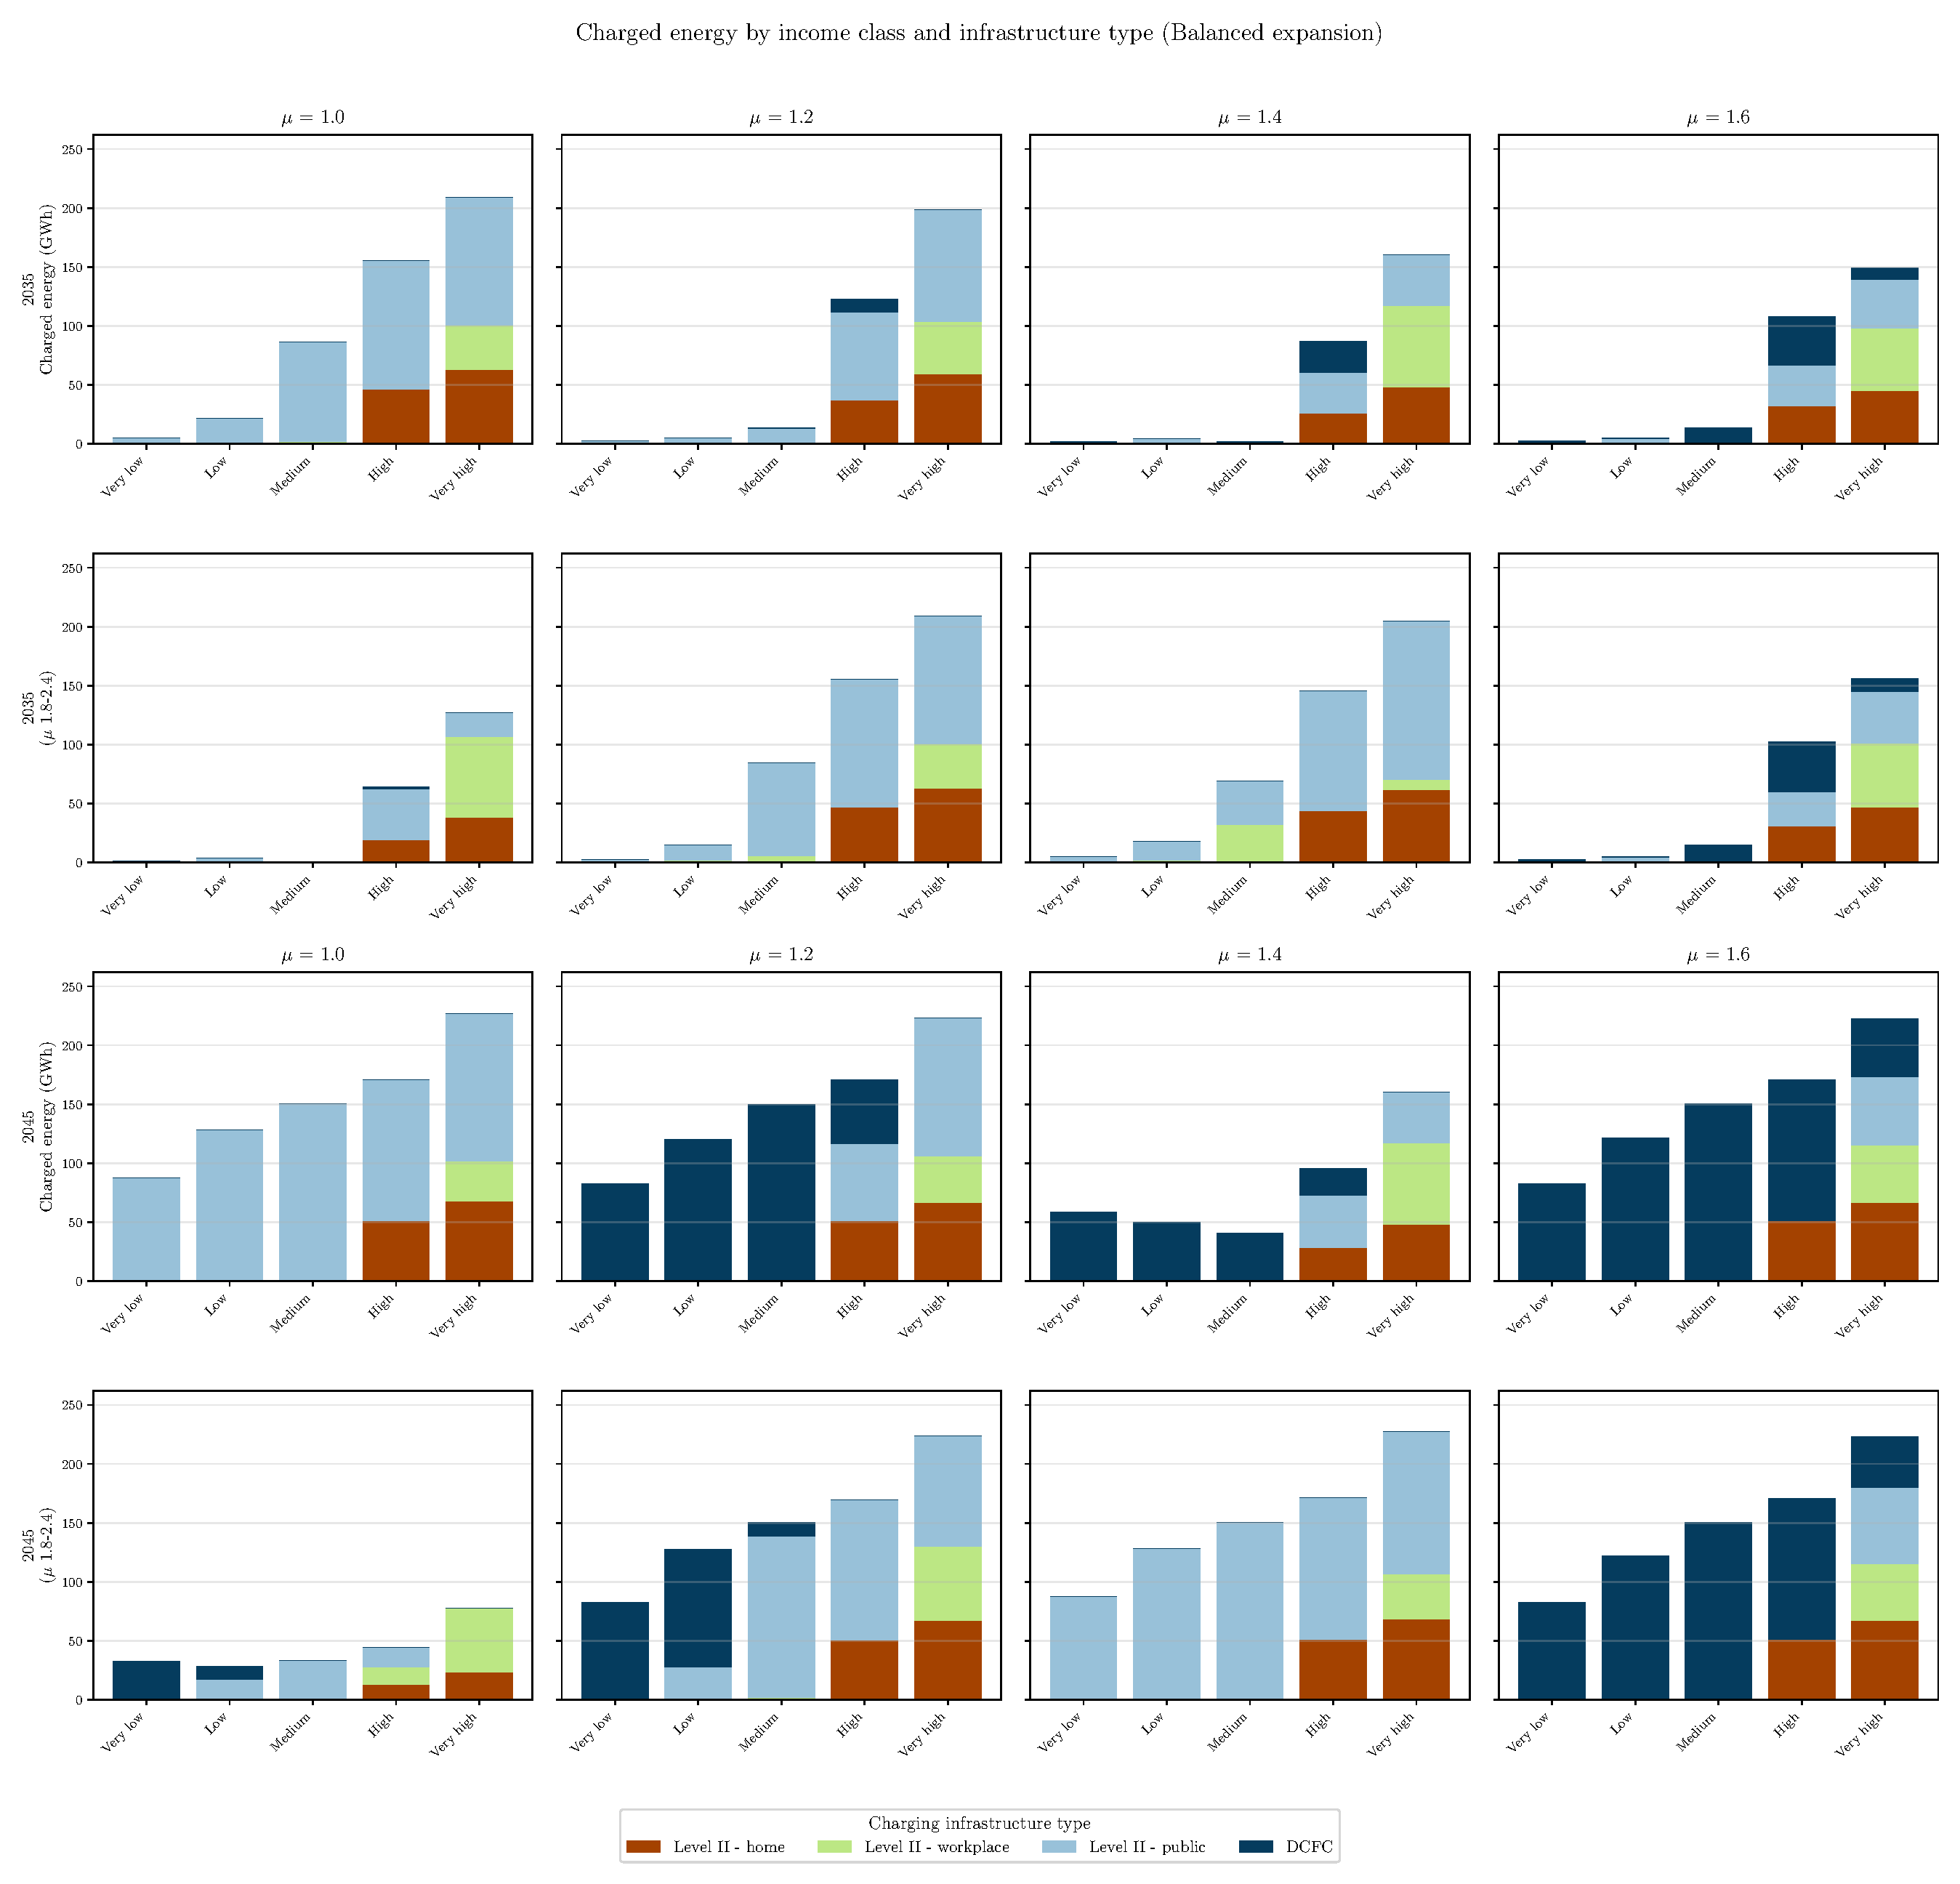
\includegraphics[width=\textwidth]{graphics/paper_2/SA_alpha_charged_energy_balanced_2026.pdf}
    \caption{Charger utilization in 2050 by income levels for different circuity values $\mu$.}\label{fig:SA_alpha_charged_energy_rq2}
\end{figure}

Figure~\ref{fig:infr_comparison_rq2} shows a negative correlation between detour times and expanded charging capacities, which is the intended behavior of the model. Higher availability of public slow charging increases adoption of the \textit{Medium low income} consumer group (Figure~\ref{fig:develop_cs_rq2}).

\begin{figure}[H]
    \centering
    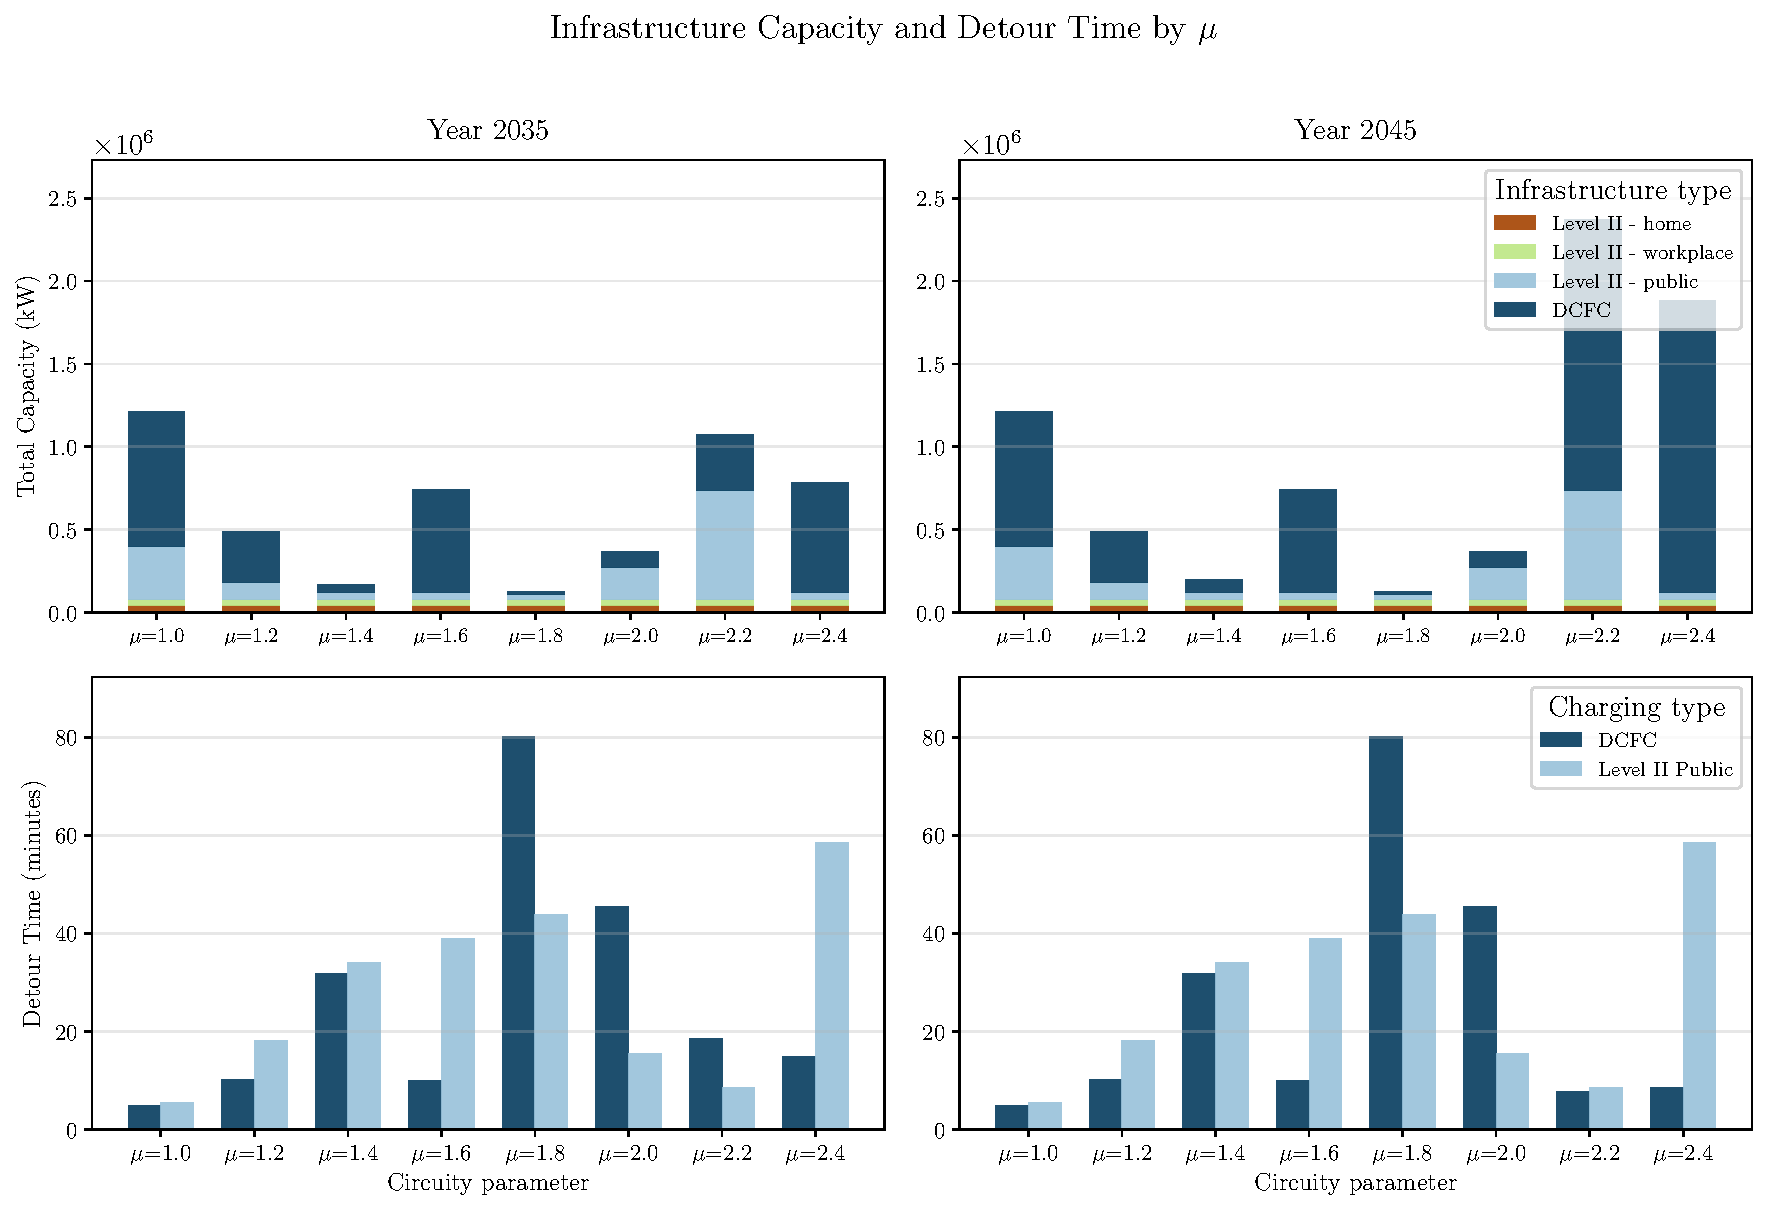
\includegraphics[width=\textwidth]{graphics/paper_2/SA_alpha_capacity_detour_combined_2026.pdf}
    \caption{Comparison of total installed charging infrastructure and average detour times for different circuity values $\mu$.}\label{fig:infr_comparison_rq2}
\end{figure}

\begin{figure}[H]
    \centering
    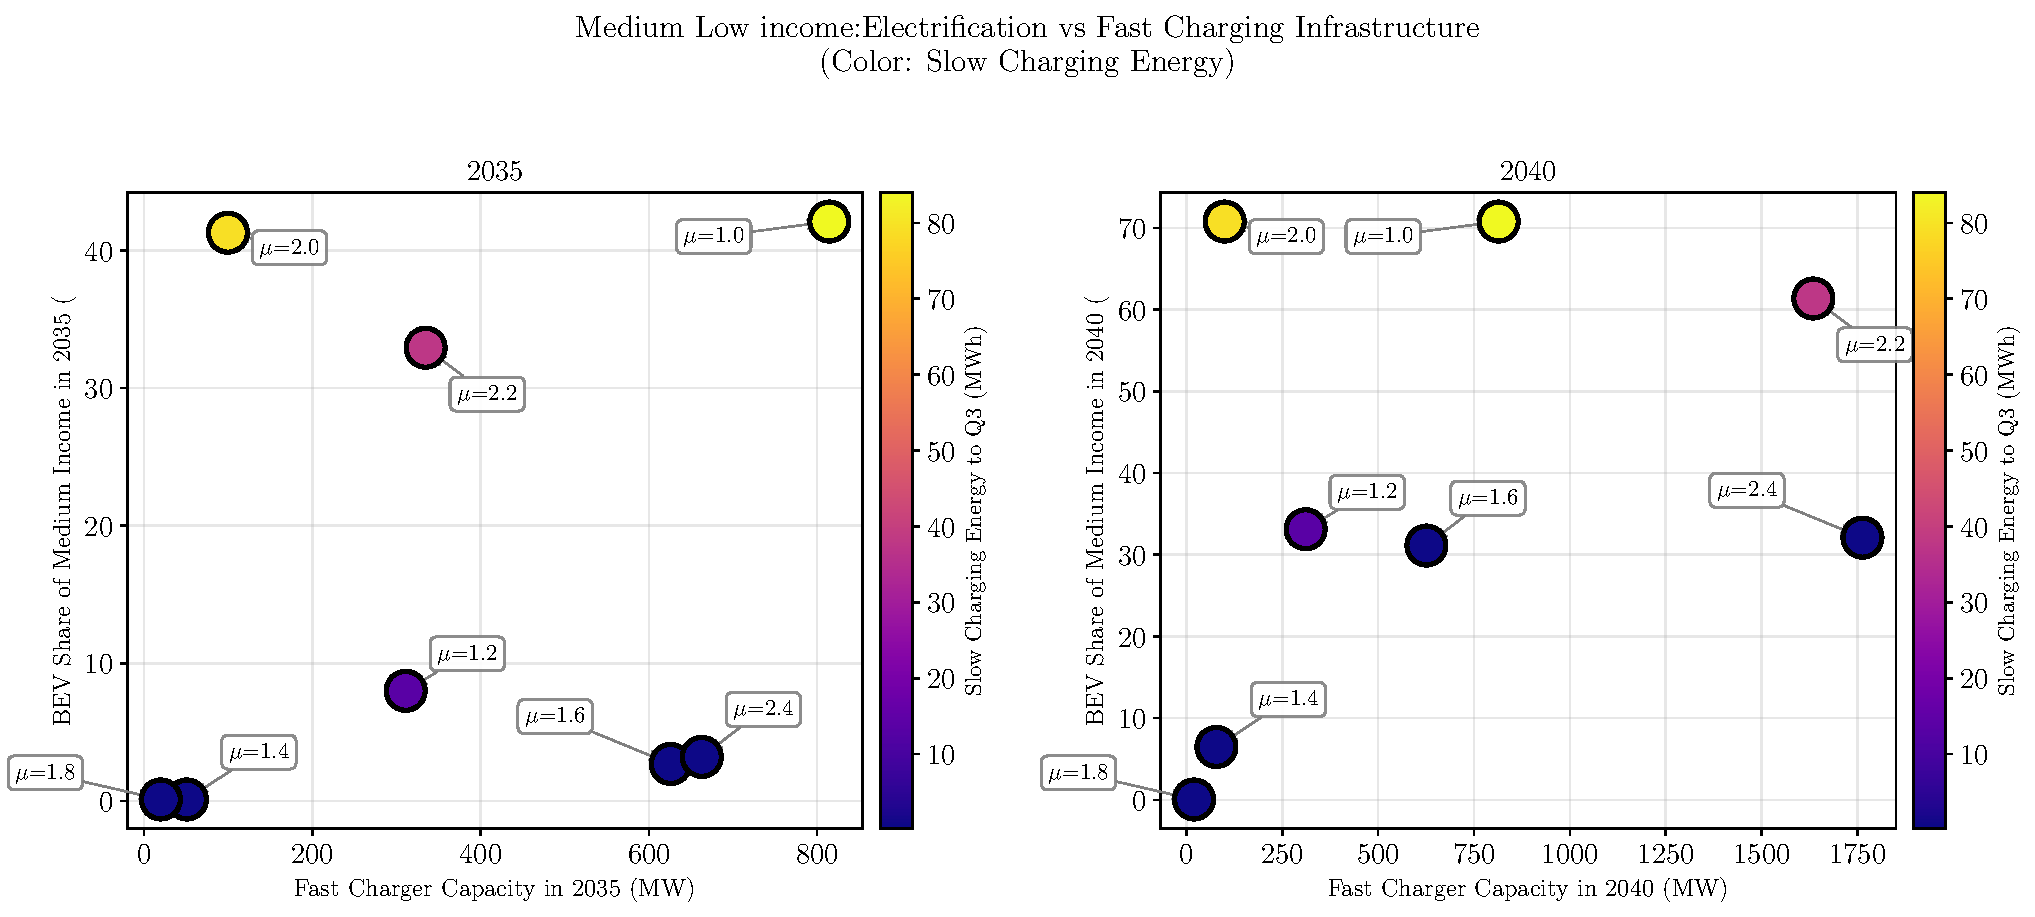
\includegraphics[width=\textwidth]{graphics/paper_2/SA_alpha_scatter_fast_colormap_slow_2035_2040.pdf}
    \caption{Fast charging capacity versus medium-income BEV adoption share for 2035 and 2040 across circuity factor sensitivity scenarios.}\label{fig:develop_cs_rq2}
\end{figure}

\section{Validation of Detour Fueling Time Function}\label{app:rq2_validation}

The assumed shape of the detour fueling time function is validated using a Monte Carlo-based approach with real charger data from OpenChargeMap \citep{openchargemap2011} and official Basque Country boundaries \citep{eurostat_gisco_nuts}. The procedure samples 1{,}000 random driver locations within the region, identifies the nearest charging station for each location, and calculates the detour time using the same circuity factor and driving speed assumptions as in the model. The validation is performed separately for slow and fast charging networks.

\begin{figure}[H]
    \centering
    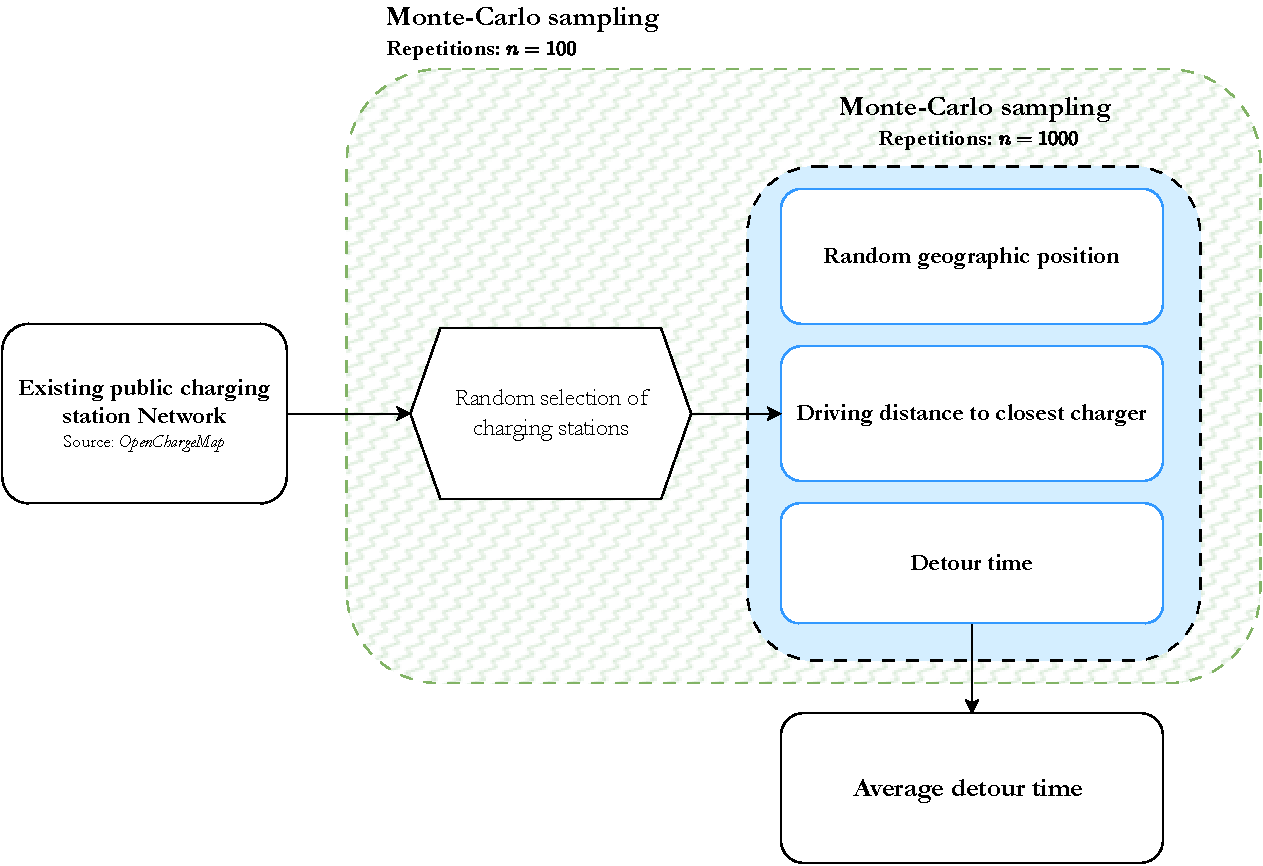
\includegraphics[width=\textwidth]{graphics/paper_2/new_algorithm.drawio.pdf}
    \caption{Overview of the sampling-based verification of detour fueling time assumptions for the Basque Country.}\label{fig:monte_carlo_sim_rq2}
\end{figure}

\begin{figure}[H]
    \centering
    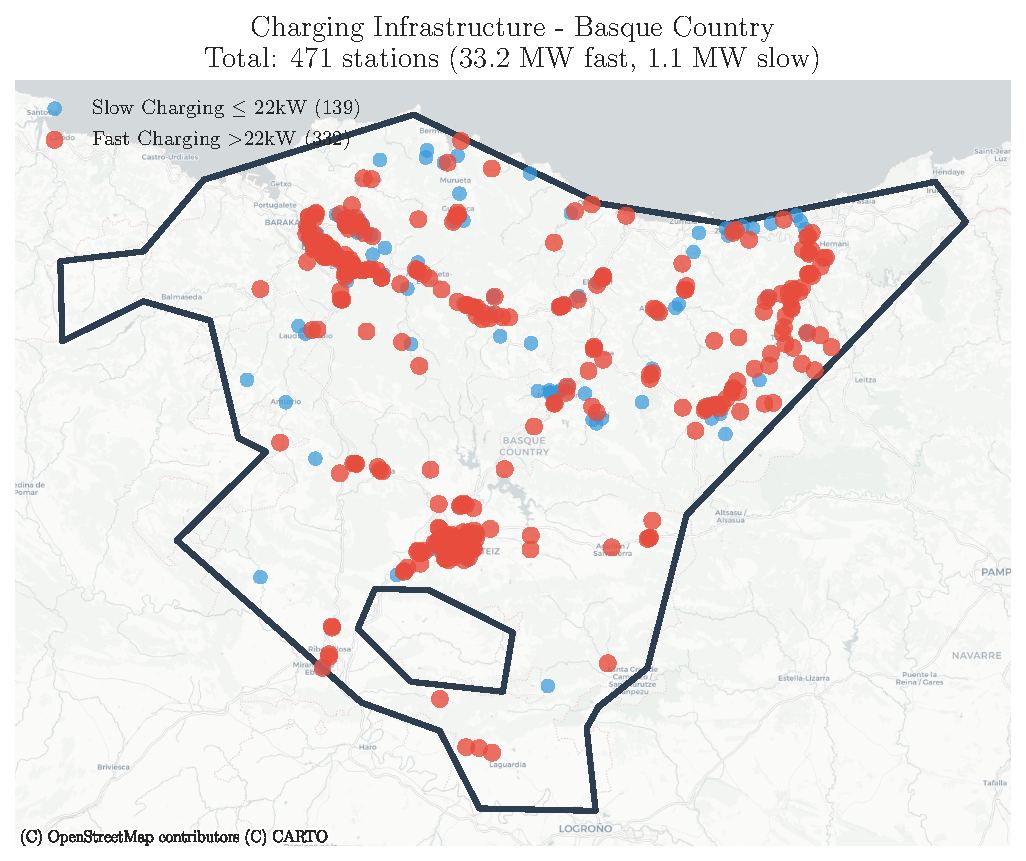
\includegraphics[width=0.8\textwidth]{graphics/paper_2/study_area_map.pdf}
    \caption{Public charger network in the Basque Country, retrieved from OpenChargeMap \citep{openchargemap2011}.}\label{fig:existing_capacity_rq2}
\end{figure}

Figures~\ref{fig:validation_slow_rq2} and~\ref{fig:validation_fast_rq2} display the validation results for slow and fast chargers, respectively. The results show strong correspondence between the analytical assumptions and the empirically-derived curves from the real charging infrastructure.

\begin{figure}[H]
    \centering
    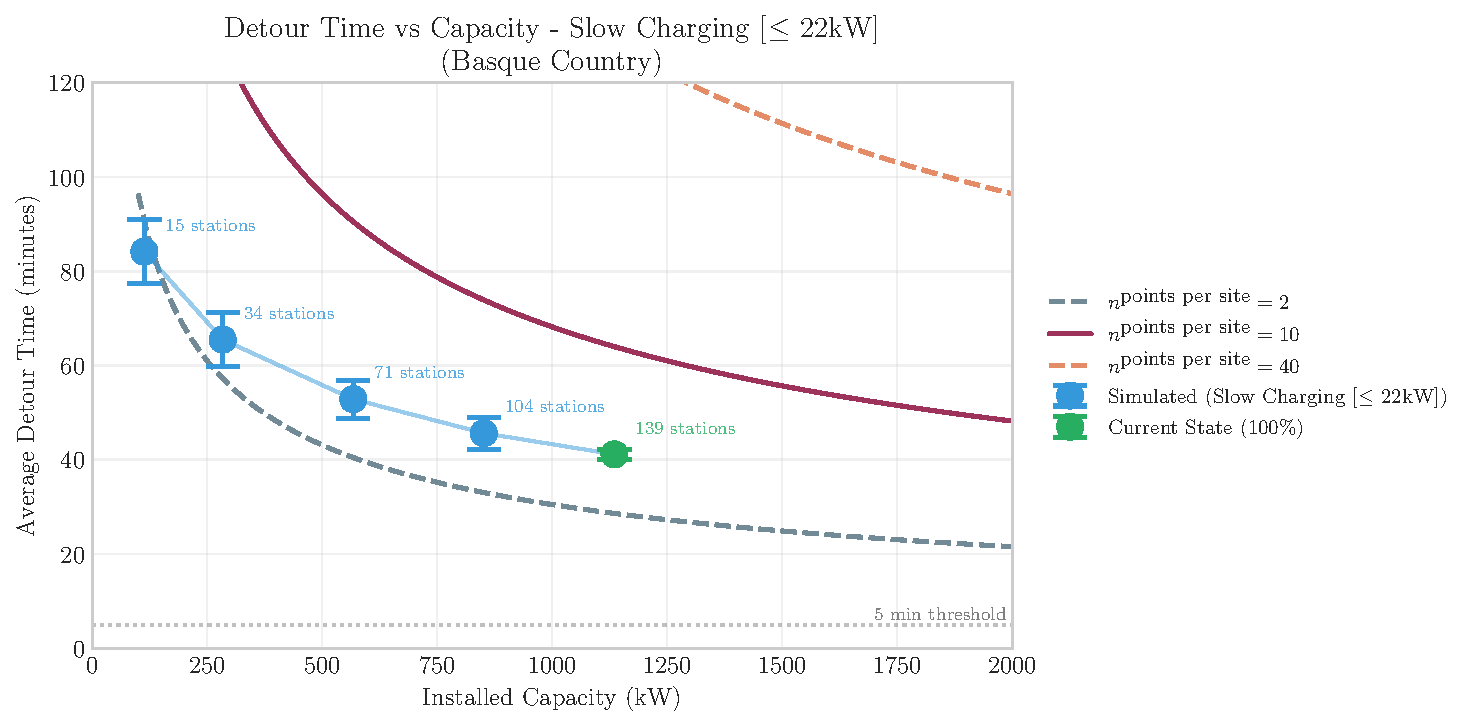
\includegraphics[width=\textwidth]{graphics/paper_2/curve_validation_slow.pdf}
    \caption{Validation of the detour fueling time function for slow chargers in the Basque Country: comparison between Monte Carlo simulation results and assumed functional form.}\label{fig:validation_slow_rq2}
\end{figure}

\begin{figure}[H]
    \centering
    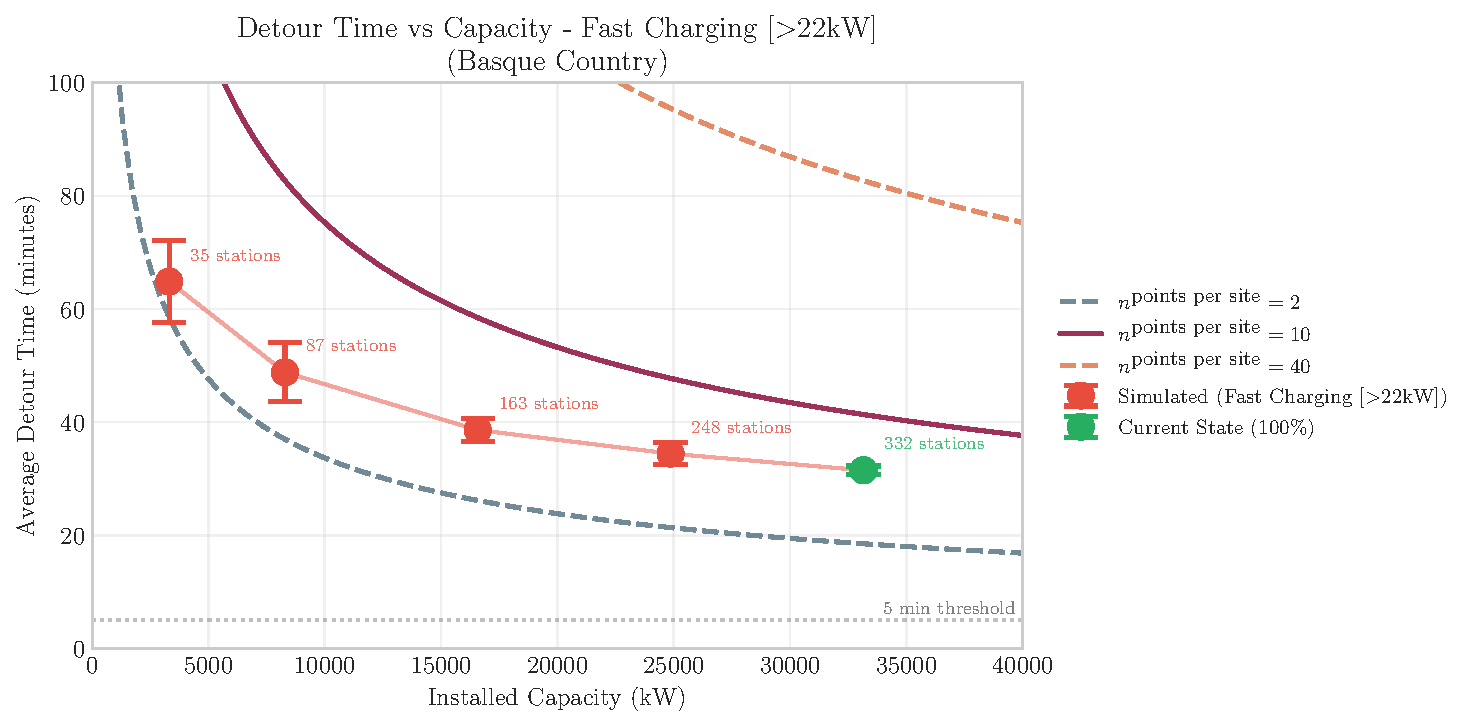
\includegraphics[width=\textwidth]{graphics/paper_2/curve_validation_fast.pdf}
    \caption{Validation of the detour fueling time function for fast chargers in the Basque Country: comparison between Monte Carlo simulation results and assumed functional form.}\label{fig:validation_fast_rq2}
\end{figure}

\section{Sensitivity Analysis: Value of Time}\label{app:rq2_vot}

The value of time (VoT) represents the monetary value that consumers assign to the time spent detouring to reach a charging station. Based on the Victoria Transport Policy Institute recommendation (50\% of hourly wage rate for personal travel), VoT values are derived for each income class. Table~\ref{tab:vot_rq2} displays the base case values, adjusted from Danish quintile data to Spanish income ratios.

\begin{table}[H]
    \centering
    \caption{Comparison of value of time estimates using Danish and Spain-adjusted income ratios.}
    \label{tab:vot_rq2}
    \begin{tabular}{lcccc}
    \toprule
    Quintile & \multicolumn{2}{c}{VoT Before} & \multicolumn{2}{c}{VoT After (Spain ratio)} \\
    \cmidrule(lr){2-3} \cmidrule(lr){4-5}
             & VoT & VoT/Avg Wage & VoT & VoT/Avg Wage \\
             & (\euro/h) & (\%) & (\euro/h) & (\%) \\
    \midrule
    Q1 & 4.37 & 17 & 3.86 & 15 \\
    Q2 & 8.45 & 33 & 8.19 & 32 \\
    Q3 & 12.53 & 49 & 12.53 & 49 \\
    Q4 & 16.61 & 65 & 16.87 & 66 \\
    Q5 & 20.69 & 81 & 21.20 & 83 \\
    \bottomrule
    \end{tabular}
\end{table}

The sensitivity analysis tests absolute shifts of $\pm 3$~\euro/h and relative compression/expansion of VoT differences between income classes (factors of 0.5, 0.75, 1.25, and 1.5). Figure~\ref{fig:vot_scenarios_rq2} illustrates the tested VoT scenarios.

\begin{figure}[H]
    \centering
    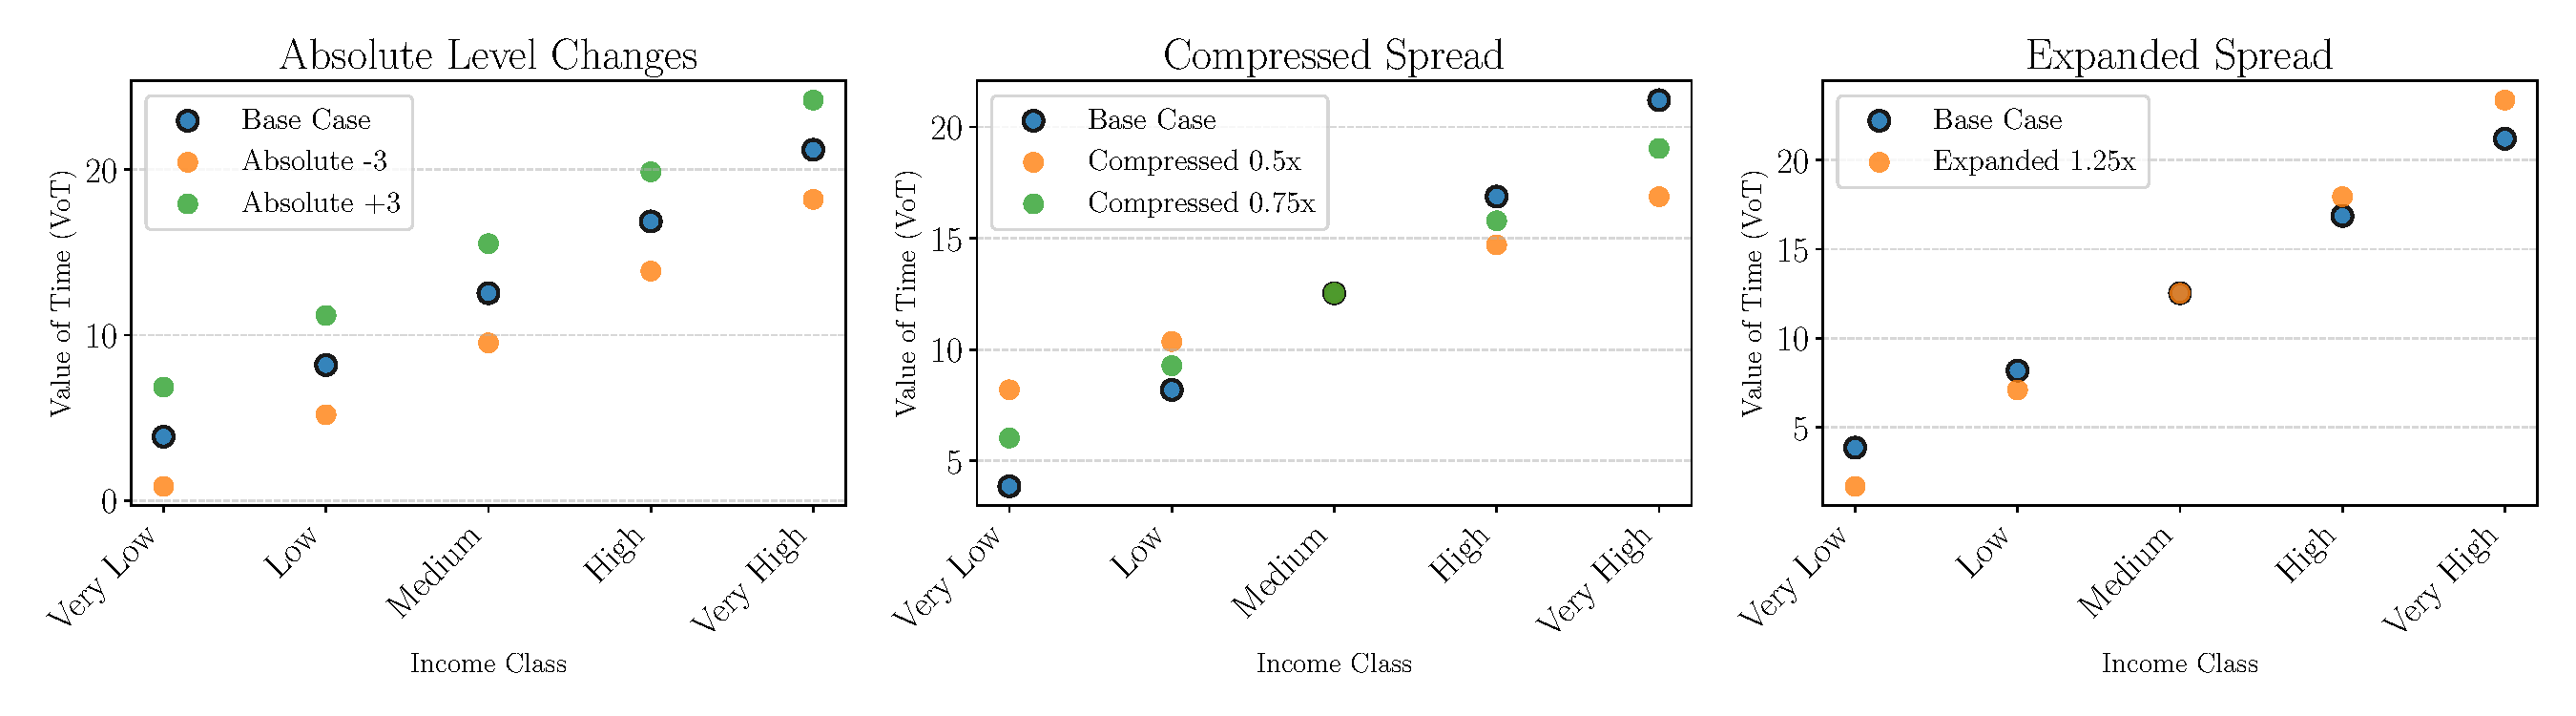
\includegraphics[width=\textwidth]{graphics/paper_2/sensitivity_analysis_vot.pdf}
    \caption{Base case VoT values for the Basque Country with tested absolute and relative changes.}\label{fig:vot_scenarios_rq2}
\end{figure}

\begin{figure}[H]
    \centering
    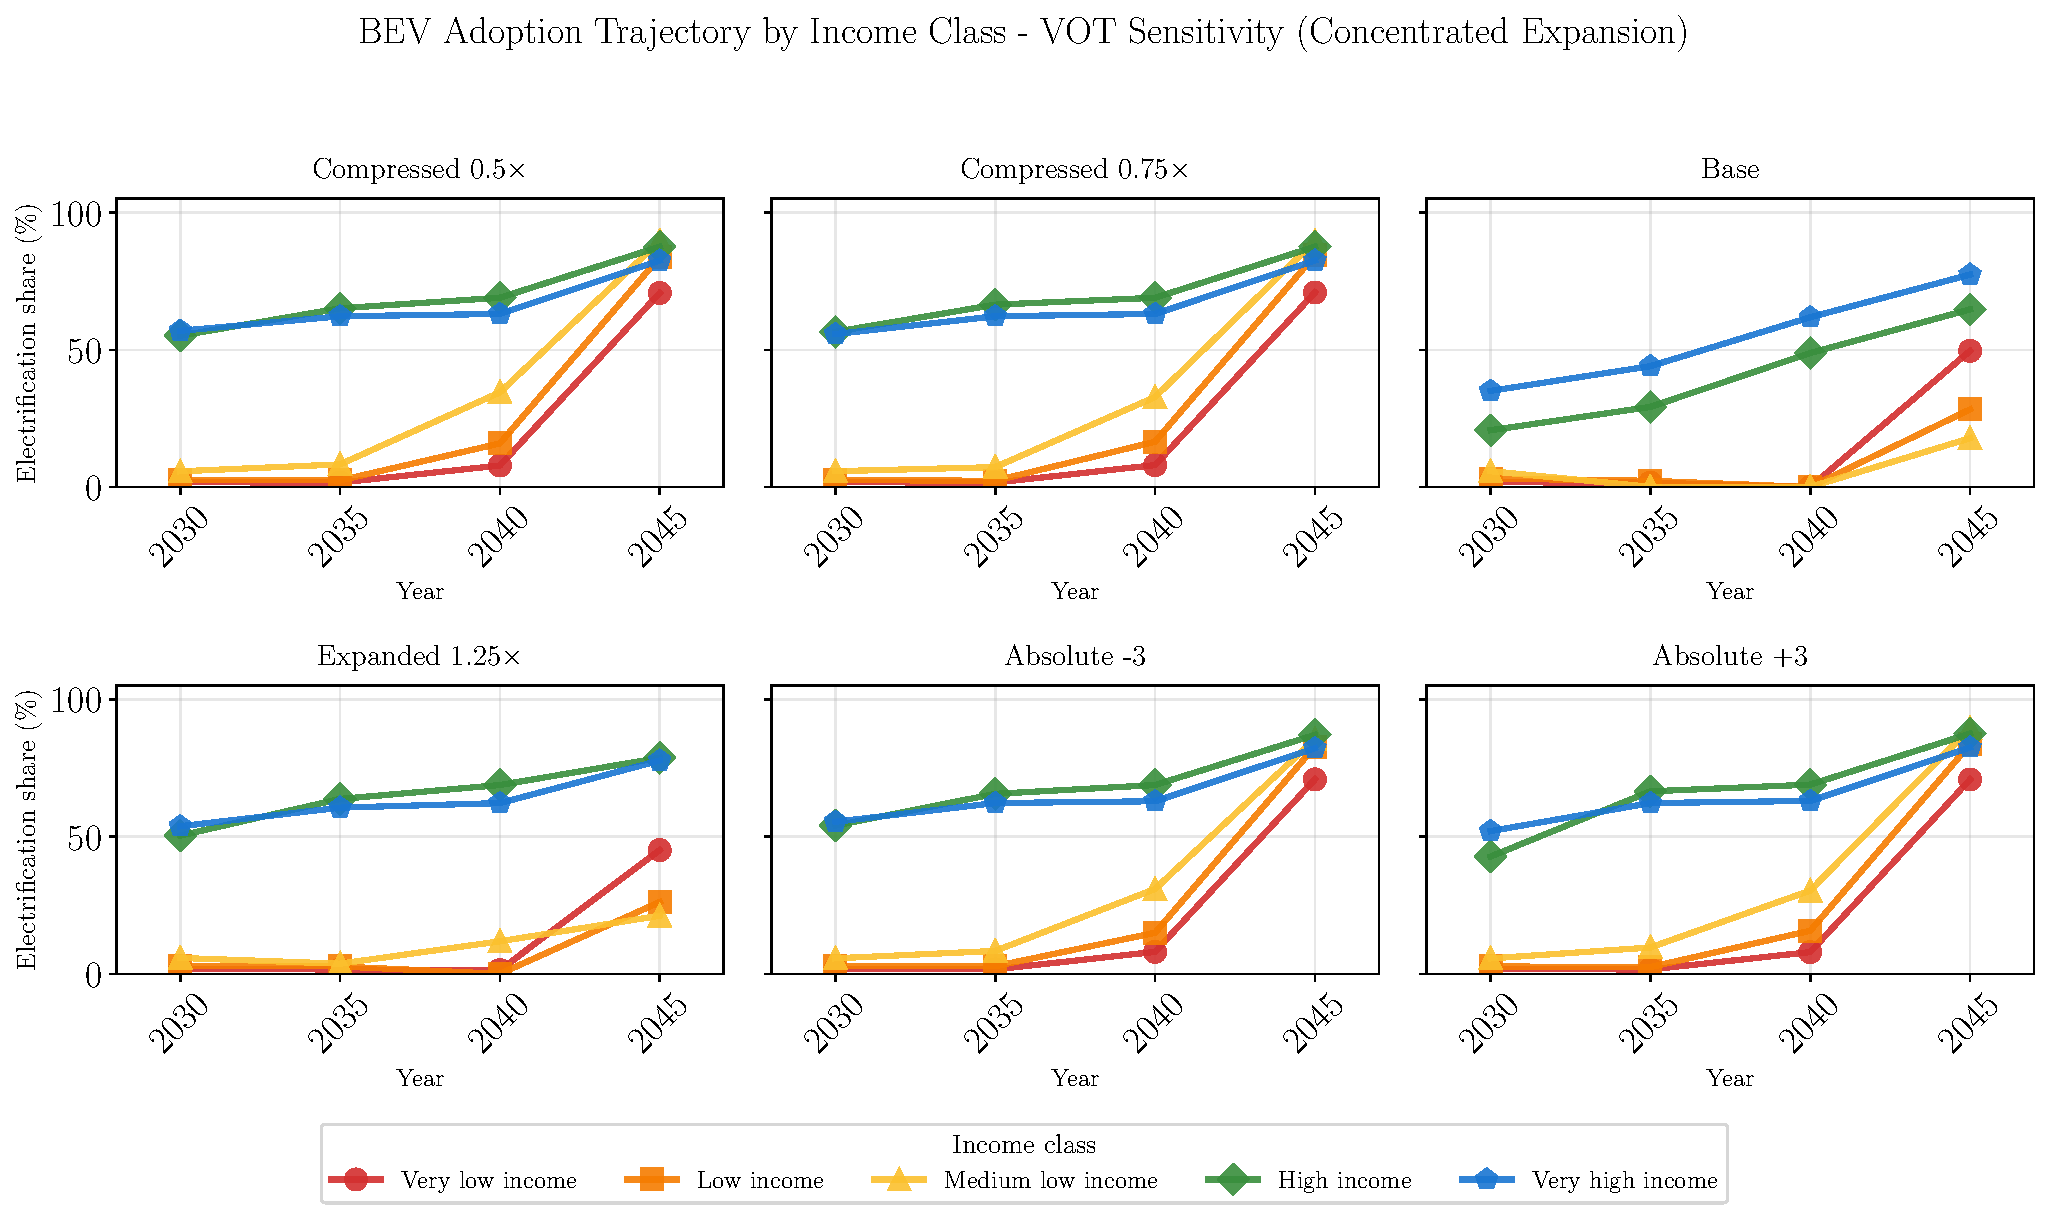
\includegraphics[width=\textwidth]{graphics/paper_2/SA_vot_bev_shares_trajectory_by_income.pdf}
    \caption{Development of electrification of the passenger car fleet by income levels during VoT sensitivity analysis.}\label{fig:vot_bevs_rq2}
\end{figure}

\begin{figure}[H]
    \centering
    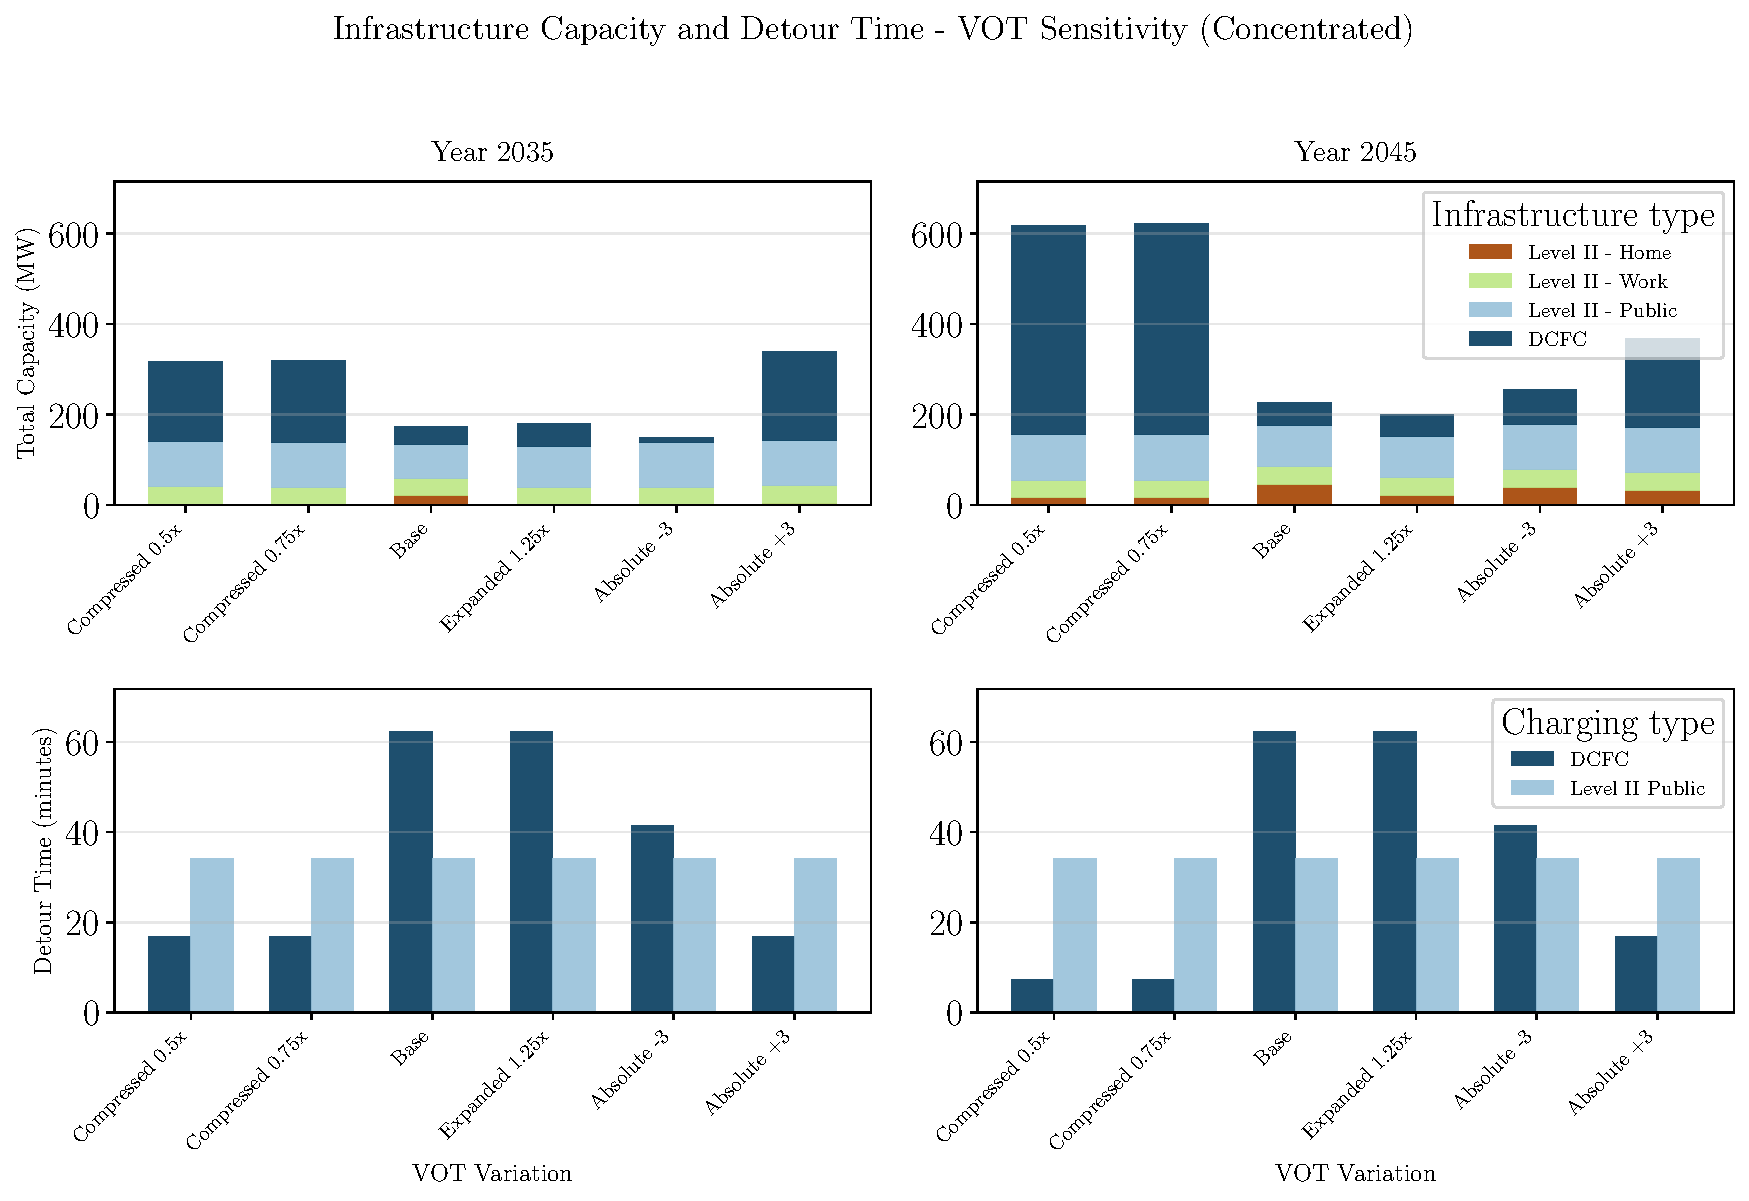
\includegraphics[width=\textwidth]{graphics/paper_2/SA_vot_capacity_detour_combined.pdf}
    \caption{Comparison of total installed charging infrastructure and average detour times for different VoT scenarios.}\label{fig:vot_infr_rq2}
\end{figure}

The highest sensitivity is observed in the \textit{Medium low income} consumer group. Fast charging utilization by the \textit{Very low income} and \textit{Low income} groups varies significantly with VoT settings.

\begin{figure}[H]
    \centering
    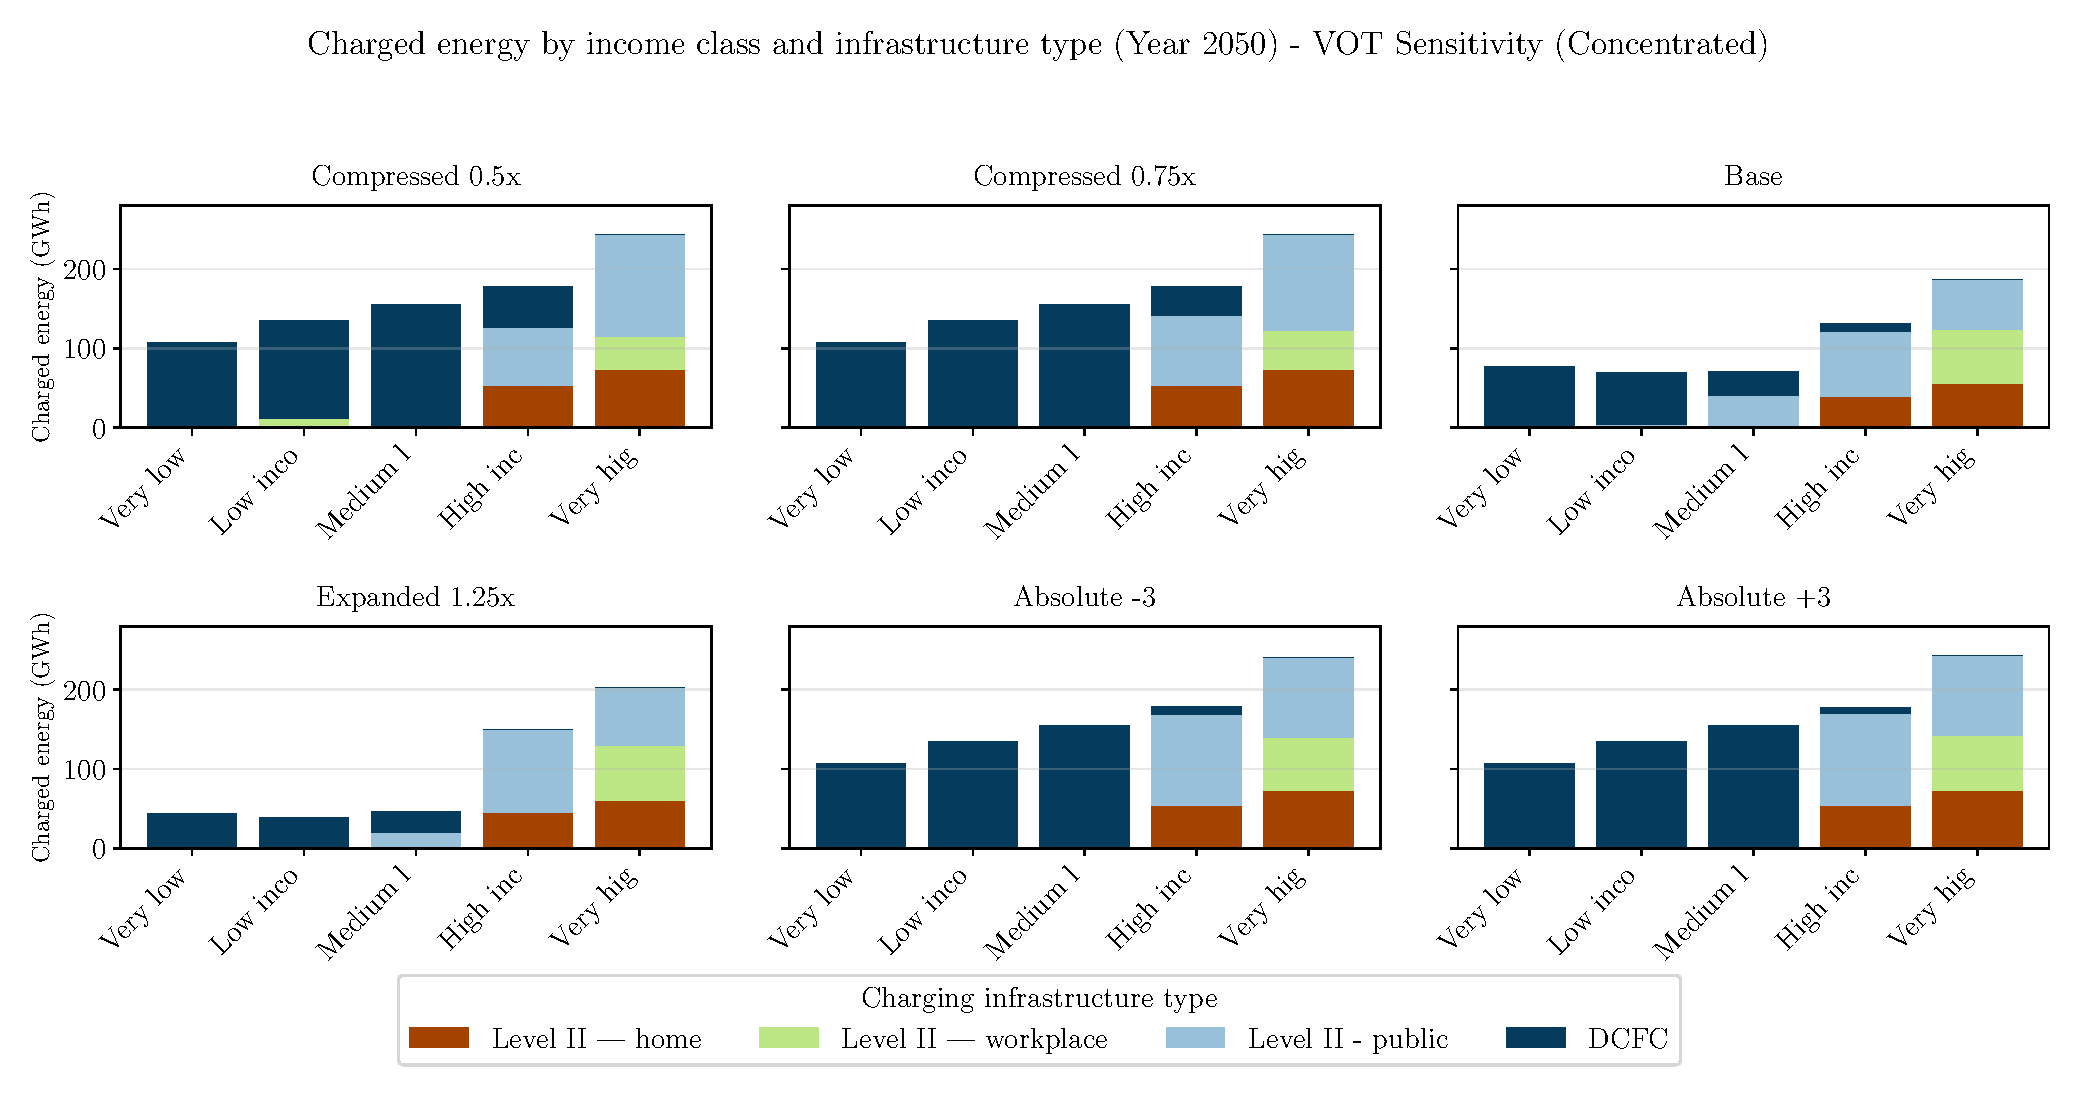
\includegraphics[width=\textwidth]{graphics/paper_2/SA_vot_charged_energy_all_scenarios.pdf}
    \caption{Charged energy by charger type in 2050 for different VoT scenarios.}\label{fig:vot_charging_rq2}
\end{figure}

\begin{figure}[H]
    \centering
    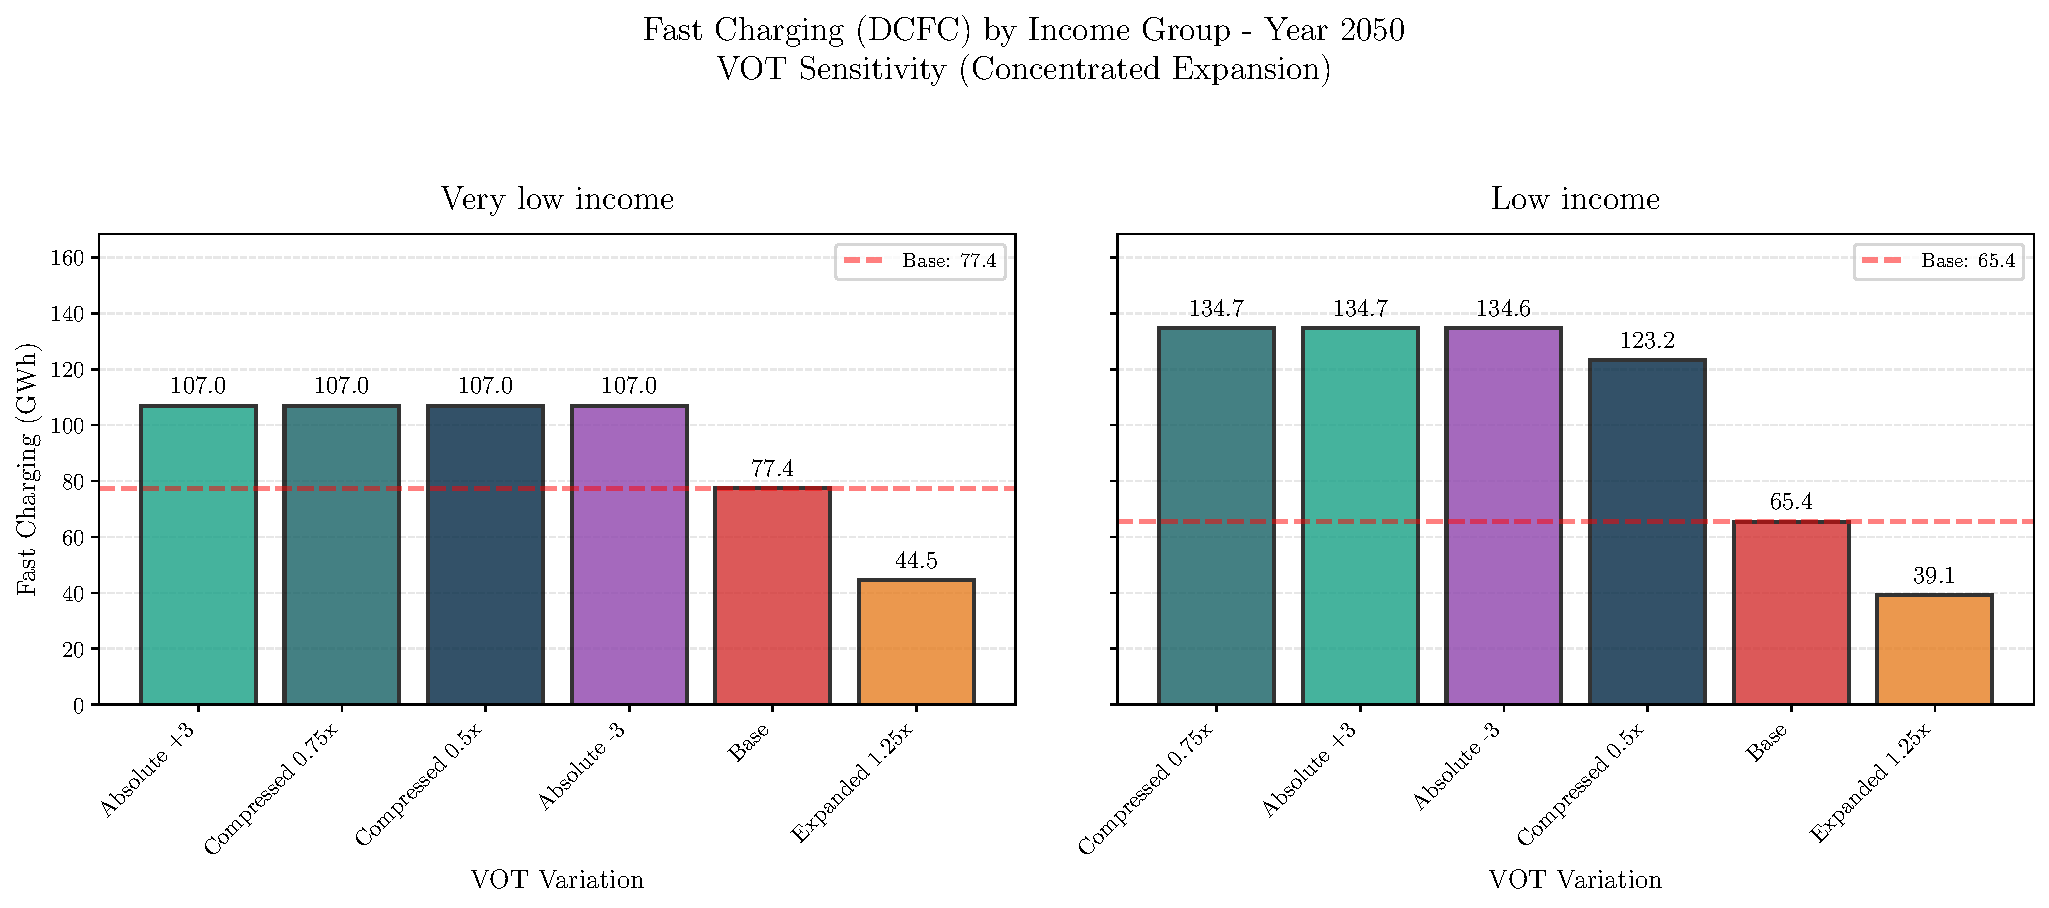
\includegraphics[width=\textwidth]{graphics/paper_2/SA_vot_fast_charging_income_comparison.pdf}
    \caption{Charged energy at fast chargers by the \textit{Very low income} and \textit{Low income} groups in 2050 for different VoT scenarios.}\label{fig:vot_fastcharg_rq2}
\end{figure}

\section{Sensitivity Analysis: Home Charger Capacities}\label{app:rq2_home}

The expansion of home charging is treated as an exogenous parameter reflecting the share of maximum home charging capacity that is reached by 2050. Five scenarios are defined: 20\%, 40\%, 60\%, 80\%, and 100\% of maximum capacity. Higher home charging availability shifts utilization away from public charging.

\begin{figure}[H]
    \centering
    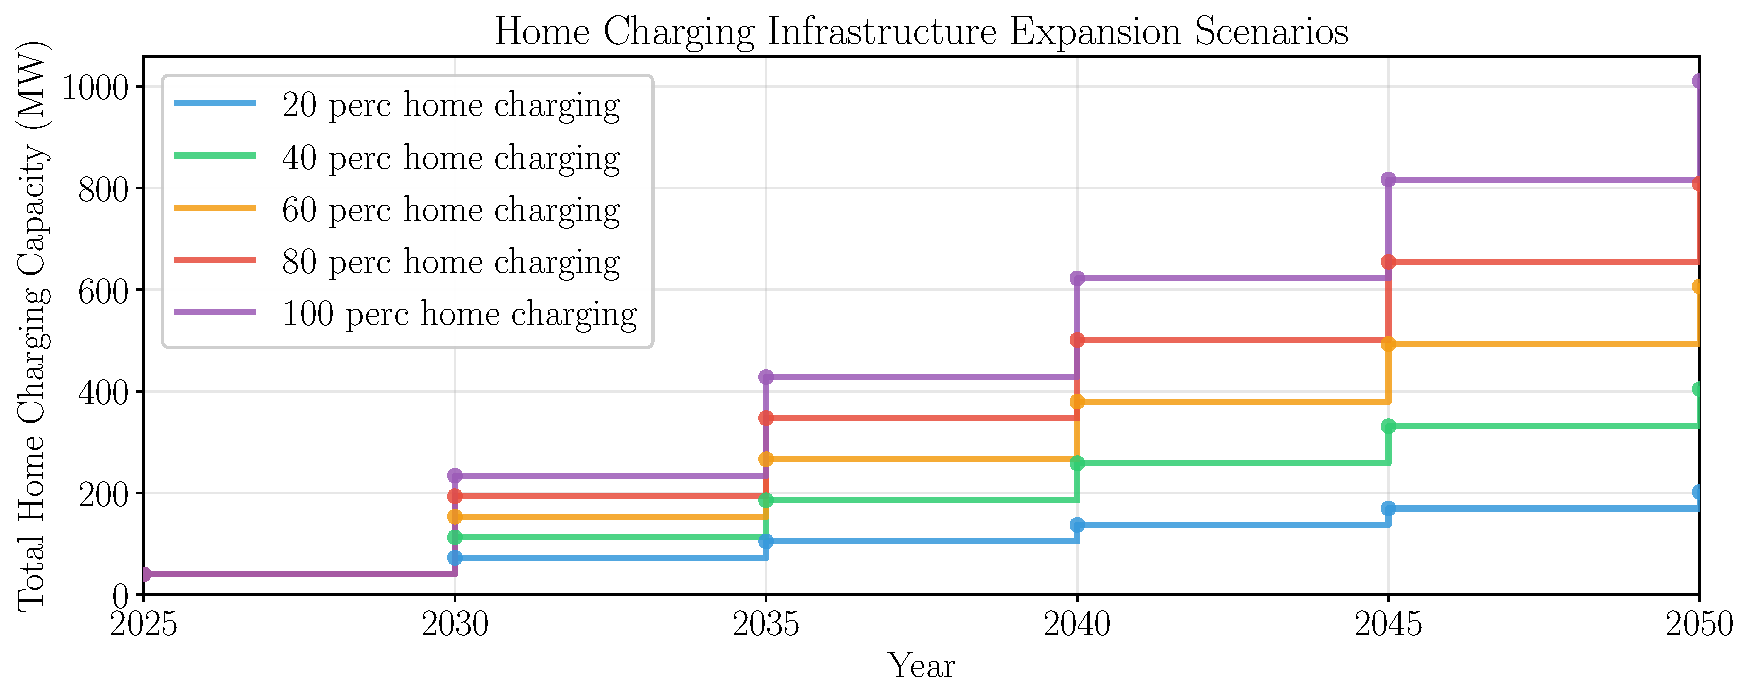
\includegraphics[width=\textwidth]{graphics/paper_2/home_charging_expansion_scenarios.pdf}
    \caption{Exogenous home charging capacity expansion scenarios.}\label{fig:home_exp_rq2}
\end{figure}

\begin{figure}[H]
    \centering
    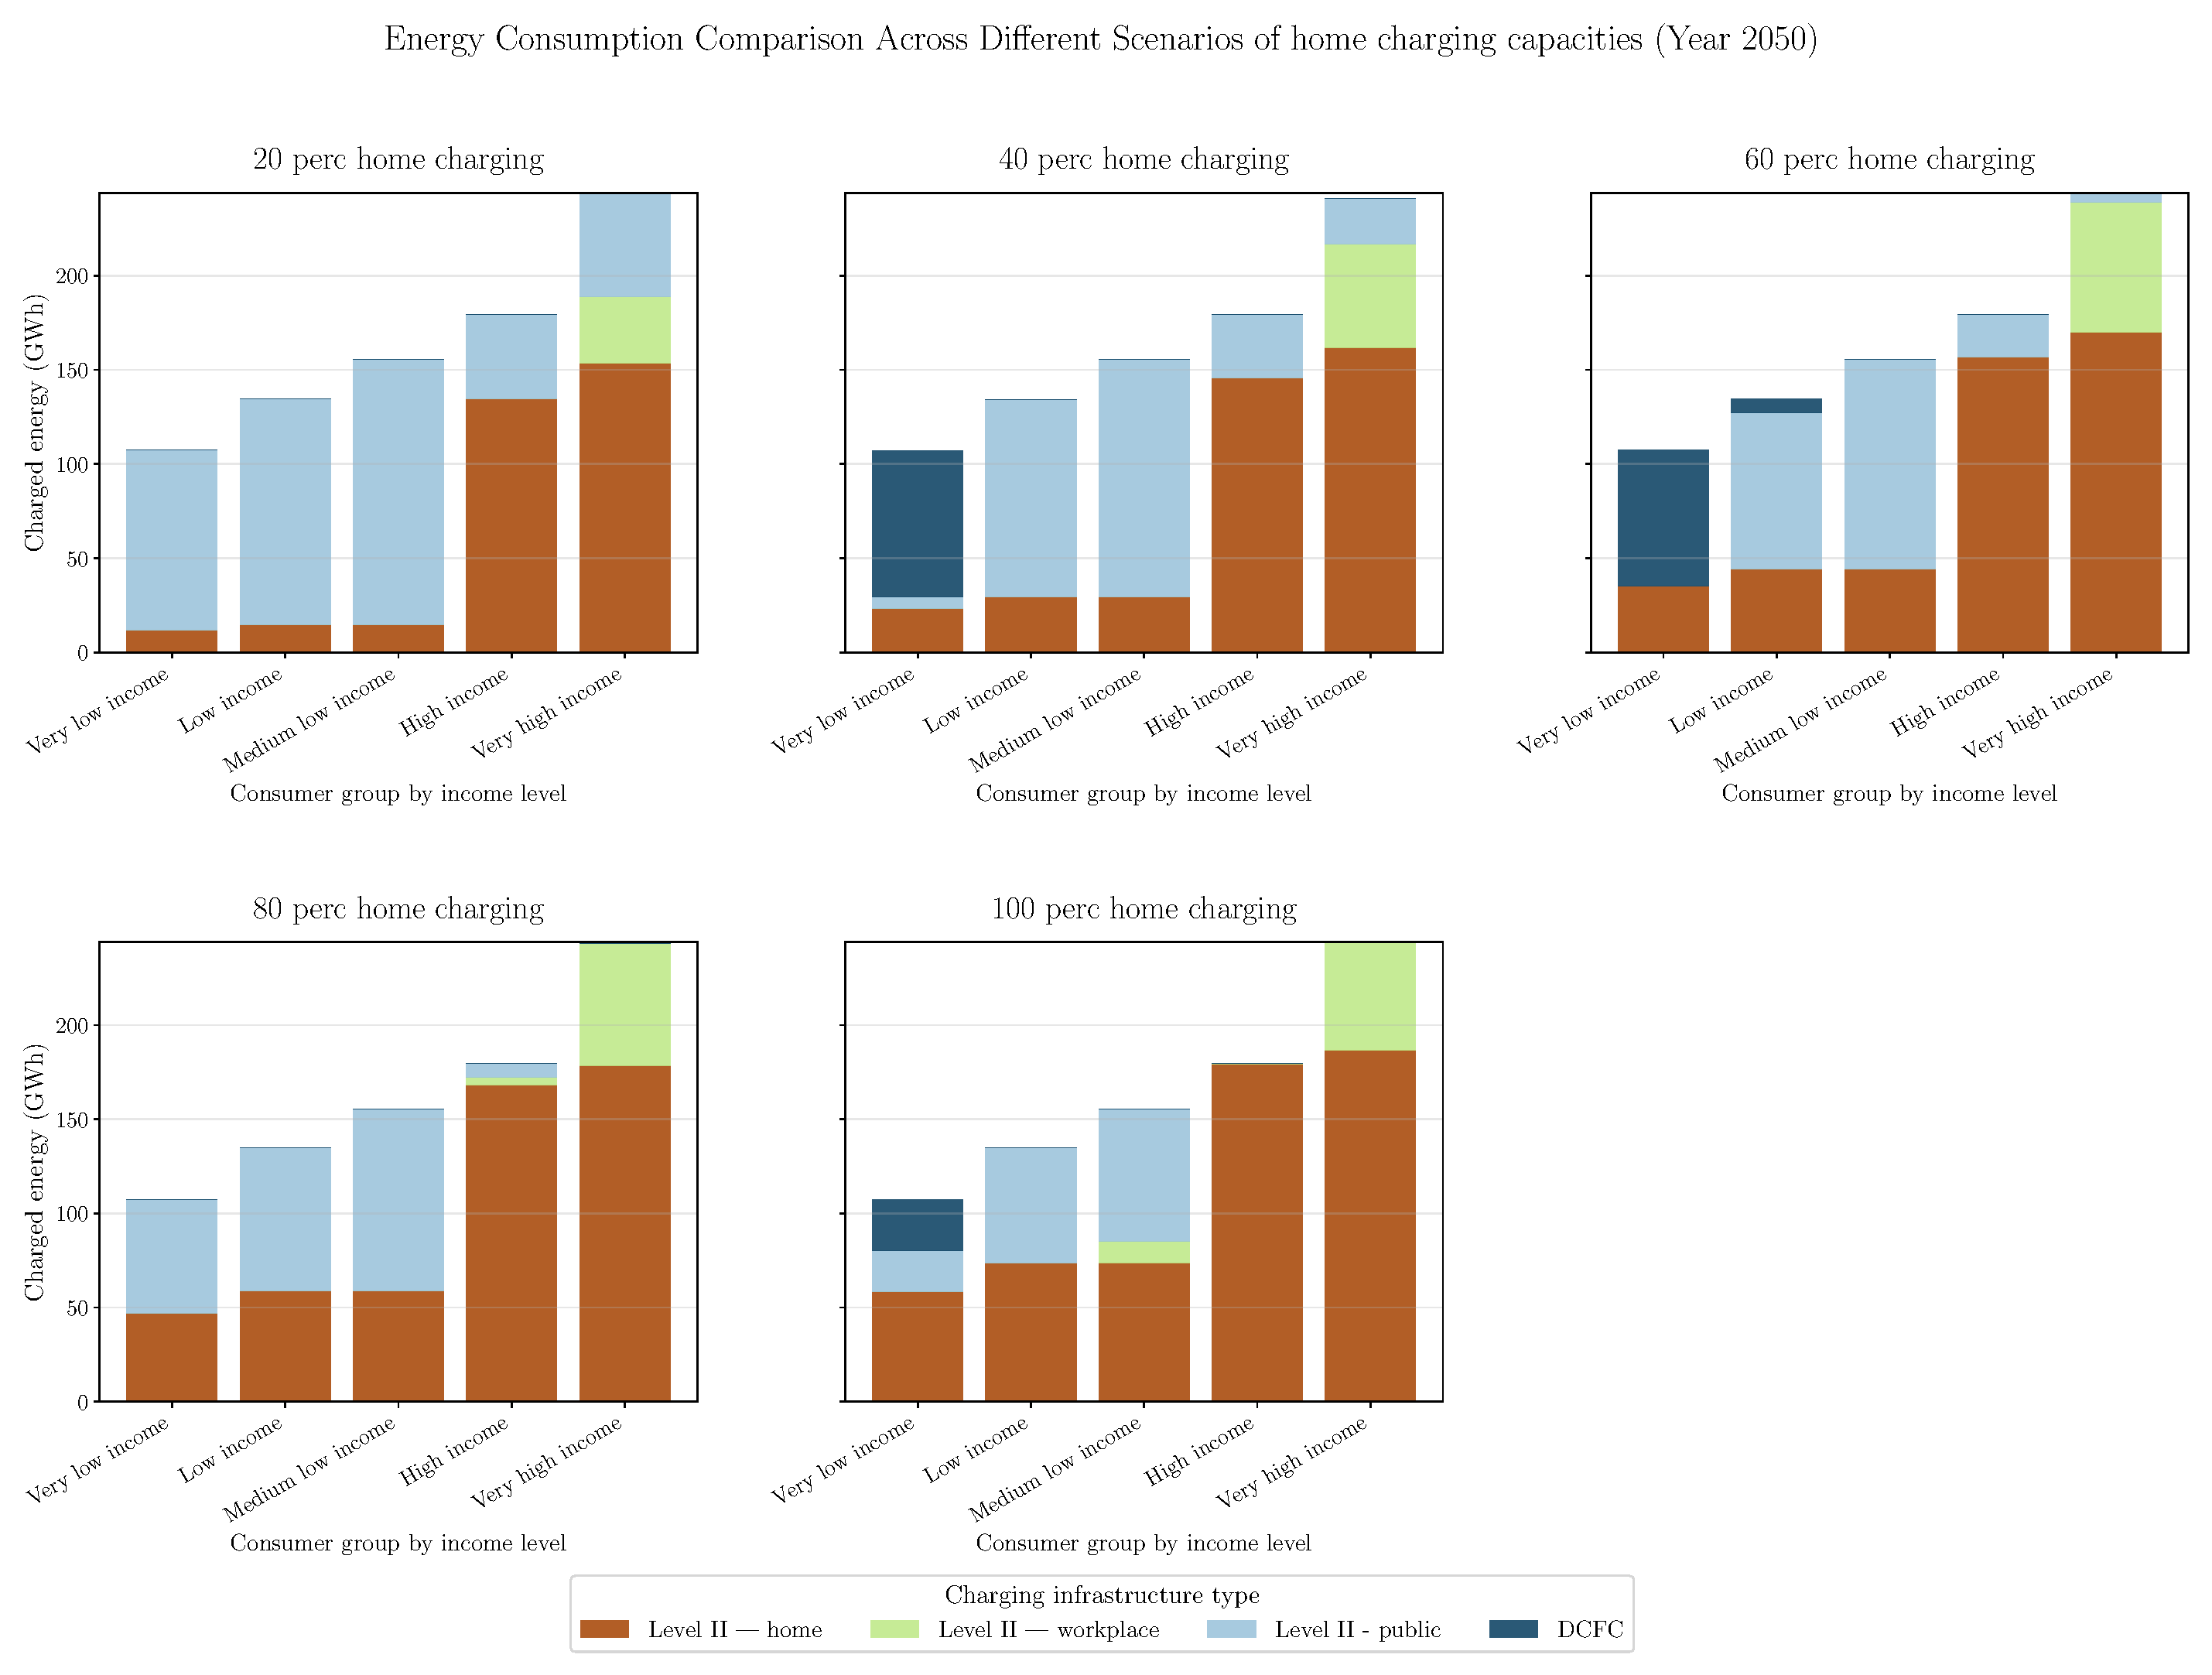
\includegraphics[width=\textwidth]{graphics/paper_2/SA_comparison_energy_consumption.pdf}
    \caption{Energy consumption patterns across income classes for different exogenous home charging capacity scenarios.}\label{fig:home_cons_rq2}
\end{figure}

\begin{figure}[H]
    \centering
    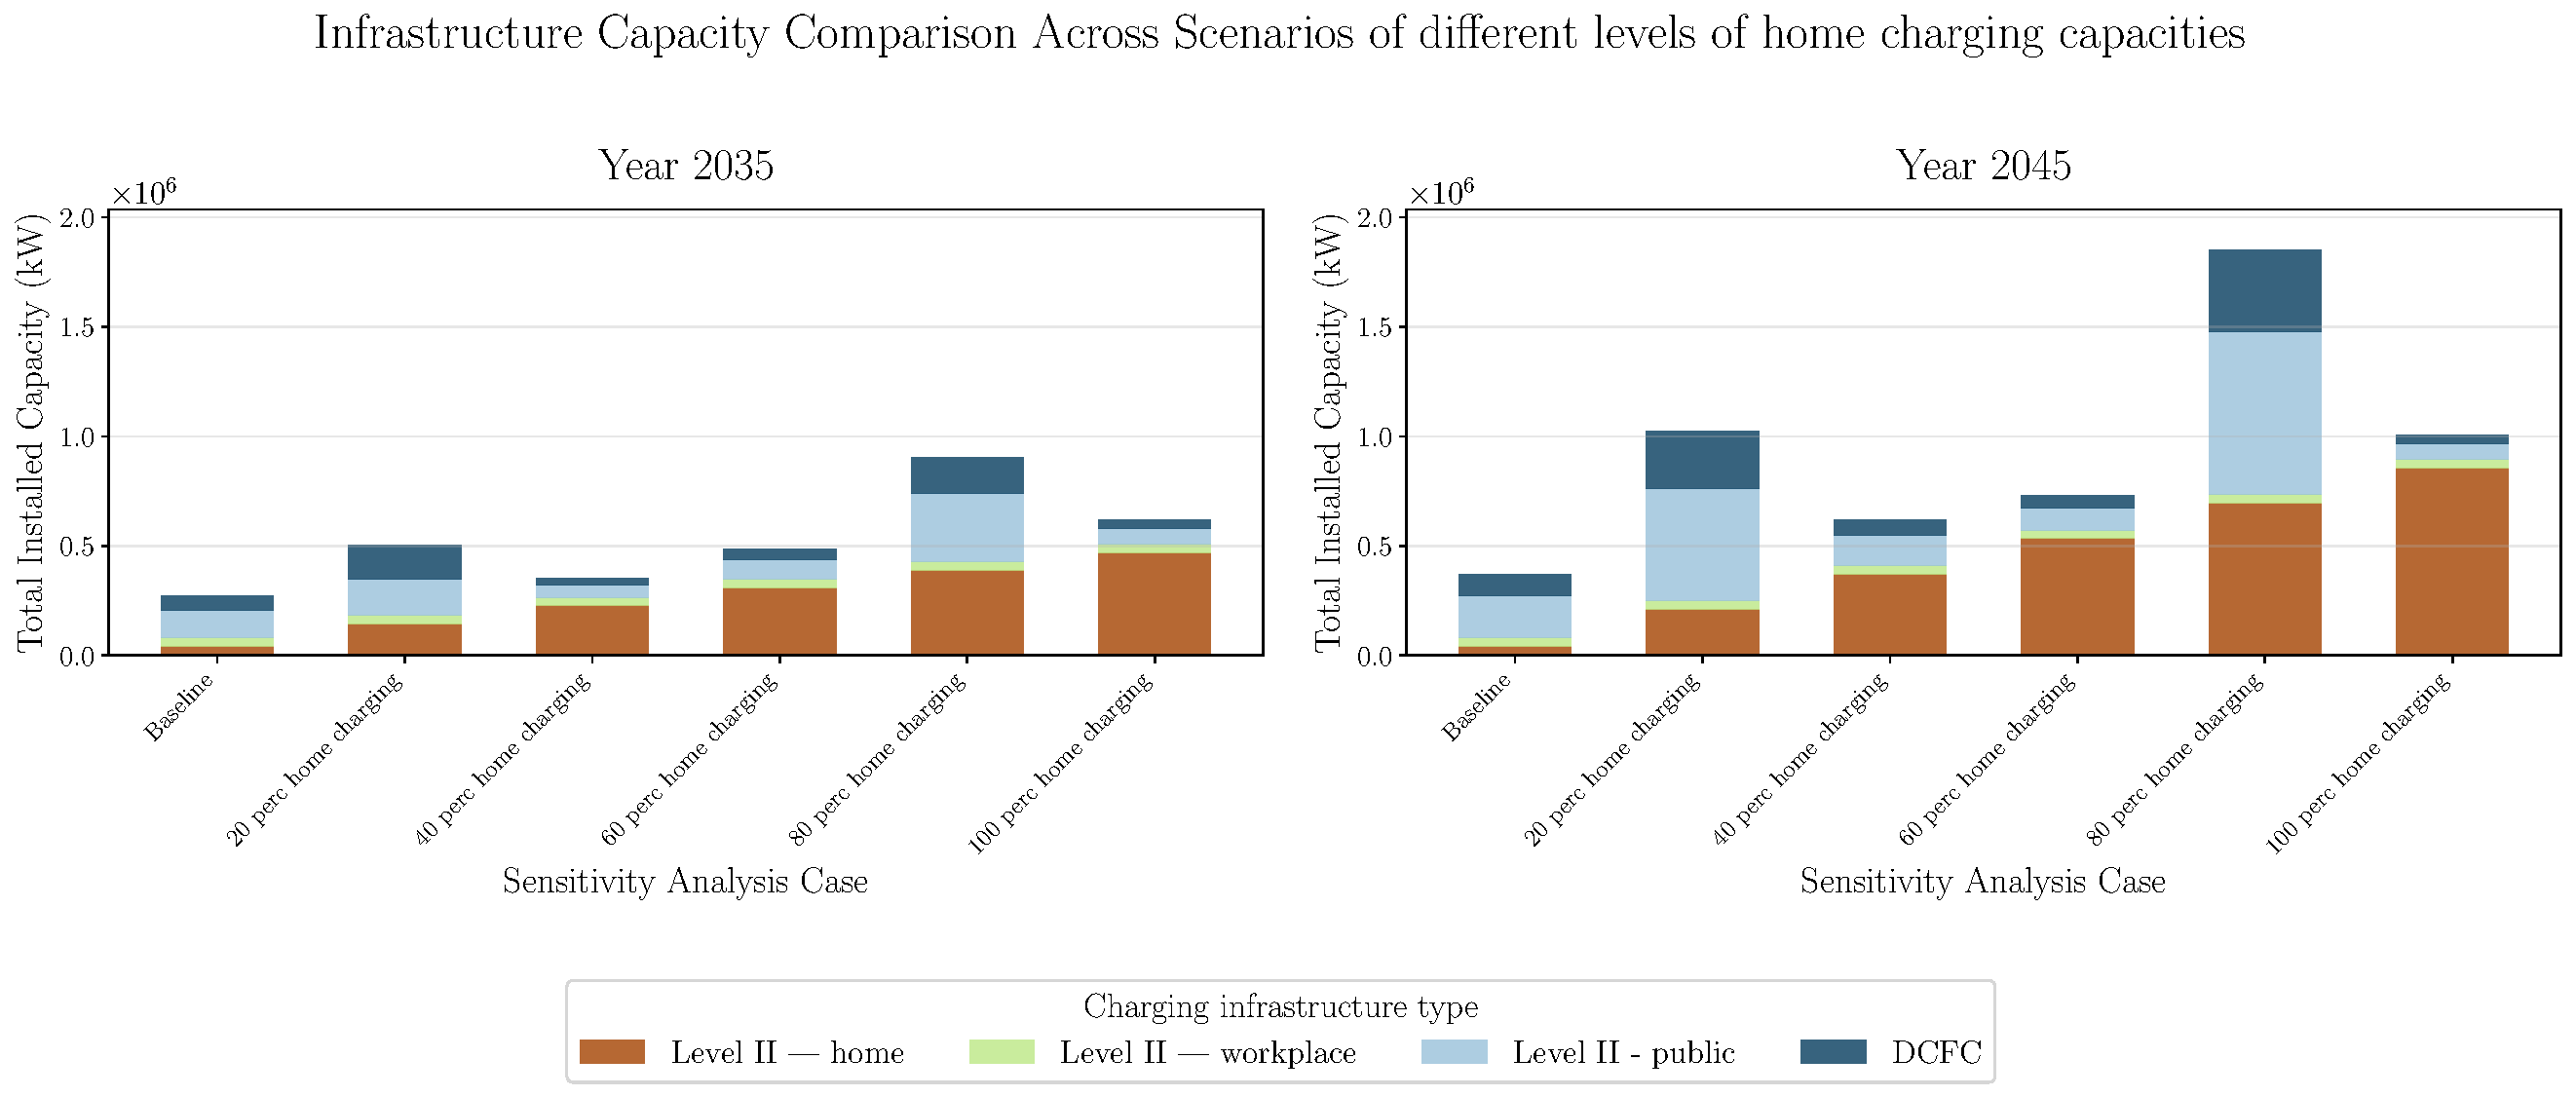
\includegraphics[width=\textwidth]{graphics/paper_2/SA_comparison_infrastructure_specific_years.pdf}
    \caption{Charging infrastructure capacities by charger type for 2035 and 2045 across home charging scenarios.}\label{fig:home_infr_rq2}
\end{figure}

\section{Sensitivity Analysis: Central Accelerated Roll-out}\label{app:rq2_spillover}

To test the robustness of the spillover effects observed in the main analysis, additional scenarios with $+15\%$, $+30\%$, and $+45\%$ capacity expansion in Bizkaia are tested. The spillover effect increases with larger capacities but remains modest overall.

\begin{figure}[H]
    \centering
    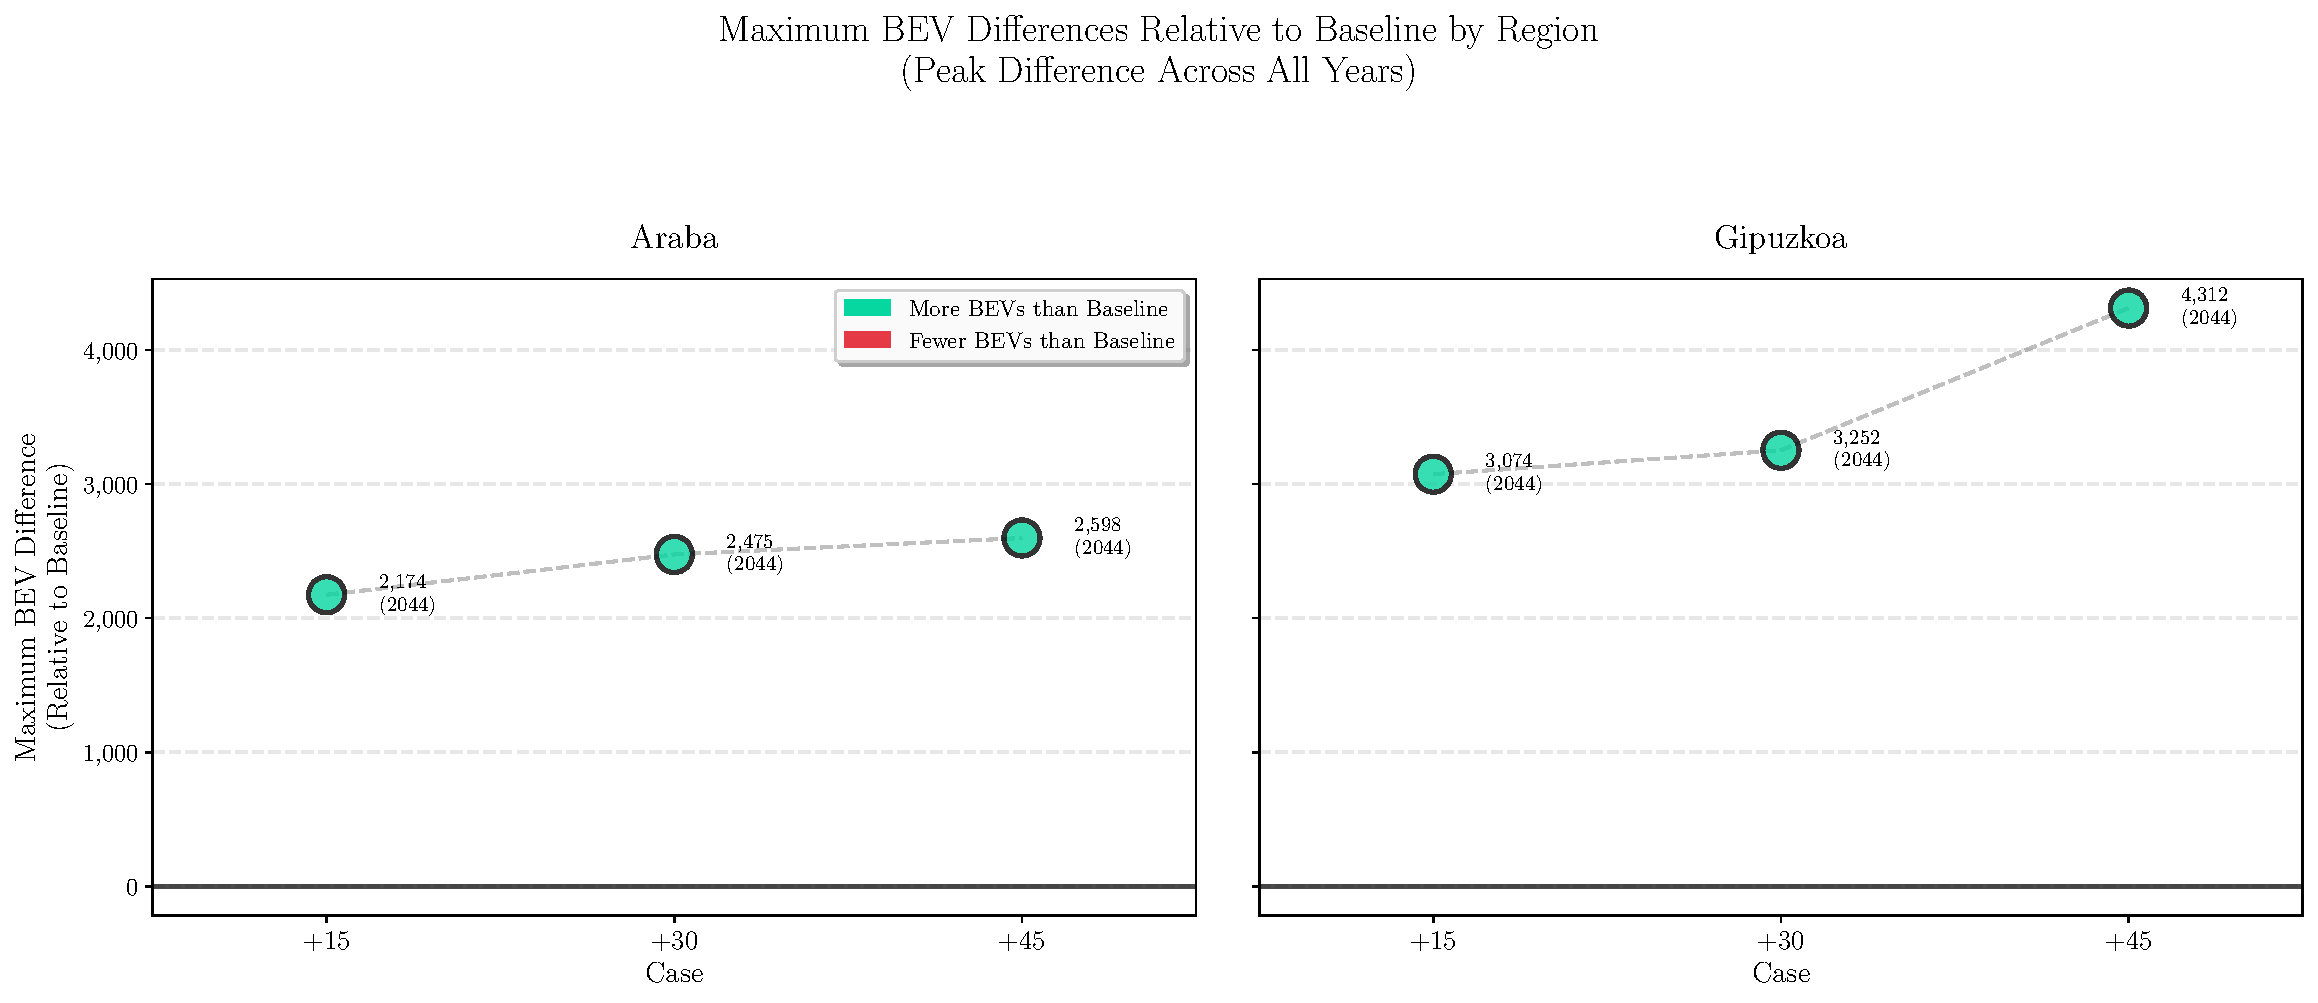
\includegraphics[width=\textwidth]{graphics/paper_2/h_comparison_maximum_bev_differences_by_region.pdf}
    \caption{Peak absolute differences in BEV adoption between the \textit{Baseline Roll-out} and \textit{Central Acc. Roll-out} scenarios across capacity expansion levels ($+15\%$, $+30\%$, $+45\%$).}\label{fig:spillover_rq2}
\end{figure}
